%%%%%%%%%%%%%%%%%%%%%%%%%%%%%%%%%%%%%%%%%%%%%%%%%%%%%%%%%%%%%%%%%%%%%%%%
%%%
%%% File: utthesis2.doc, version 2.0jab, February 2002
%%%
%%% Based on: utthesis.doc, version 2.0, January 1995
%%% =============================================
%%% Copyright (c) 1995 by Dinesh Das.  All rights reserved.
%%% This file is free and can be modified or distributed as long as
%%% you meet the following conditions:
%%%
%%% (1) This copyright notice is kept intact on all modified copies.
%%% (2) If you modify this file, you MUST NOT use the original file name.
%%%
%%% This file contains a template that can be used with the package
%%% utthesis.sty and LaTeX2e to produce a thesis that meets the requirements
%%% of the Graduate School of The University of Texas at Austin.
%%%
%%% All of the commands defined by utthesis.sty have default values (see
%%% the file utthesis.sty for these values).  Thus, theoretically, you
%%% don't need to define values for any of them; you can run this file
%%% through LaTeX2e and produce an acceptable thesis, without any text.
%%% However, you probably want to set at least some of the macros (like
%%% \thesisauthor).  In that case, replace "..." with appropriate values,
%%% and uncomment the line (by removing the leading %'s).
%%%
%%%%%%%%%%%%%%%%%%%%%%%%%%%%%%%%%%%%%%%%%%%%%%%%%%%%%%%%%%%%%%%%%%%%%%%

\documentclass[a4paper, 12pt, oneside]{report}    	%% LaTeX2e document.
\usepackage {tcdthesis}              								%% Preamble.
\usepackage{graphicx,color}
\usepackage[table]{xcolor}
\usepackage{anysize}
\usepackage{amsmath}
\usepackage{pgfplots}
\pgfplotsset{compat=1.8}
\usepackage{lmodern}
\usepackage{caption}
\usepackage{url}
\usepackage{hyperref}
\usepackage{graphicx}
\usepackage{adjustbox}
\usepackage{placeins}
\usepackage{bbding}
\usepackage{array}
\newcolumntype{P}[1]{>{\centering\arraybackslash}p{#1}}
\usepackage[parfill]{parskip}
\graphicspath{ {images/} }

\hyphenation{human measuring several students participant elevator complexity optimal problems}

\leftchapter                       							%% Uncomment one of these if you want  
%\centerchapter                      					%% left-justified, centered or
% \rightchapter                     						%% right-justified chapter headings.
                                     								%% Chapter headings includes the
                                     								%% Contents, Acknowledgments, Lists
                                     								%% of Tables and Figures and the Vita.
                                     								%% The default is \centerchapter.

% \singlespace                       					%% Uncomment one of these if you want
% \oneandhalfspace                   				%% single-spacing, space-and-a-half
 \doublespace                       						%% or double-spacing; the default is
                                     								%% \oneandhalfspace, which is the
                                     								%% minimum spacing accepted by the
                                     								%% Graduate School.

\renewcommand{\thesisauthor}{Michael Christian Frick}
\renewcommand{\thesismonth}{September}             			%% Your month of graduation.
\renewcommand{\thesisyear}{2016}                     				%% Your year of graduation.
\renewcommand{\thesistitle}{\large{Learning Processes and Consistency in the Quality of Software Development Based on Environmental Influences} }
\renewcommand{\thesisauthorpreviousdegrees}{B.Sc.}  		%% Your previous degrees, abbreviated; separate multiple degrees by commas.
\renewcommand{\thesissupervisor}{Stephen Barrett}

\renewcommand{\thesisauthoraddress}{Dublin, Ireland}
\renewcommand{\thesisdegree}{Master of Science in Computer Science}
\renewcommand{\thesisdegreeabbreviation}{M.Sc.}
\renewcommand{\thesistype}{Dissertation}

                                     
%%%%%%%%%%%%%%%%%%%% BEGIN THE DOCUMENT %%%%%%%%%%%%%%%%%%%%%%%%%%%%%%%%%%%%%%%%%%%%
\begin{document}

\thesistitlepage                                  		%% Generate the title page.
\thesisdeclarationpage									%% Generate the declaration page.
\thesispermissionpage									%% Generate the copyright permission page

\begin{thesisacknowledgments}               	%% Use this to write your
			                          							%% acknowledgments; it can be anything
Give many thanks and stuff...

\end{thesisacknowledgments}                   %% allowed in LaTeX2e par-mode.

\begin{thesisabstract}
\section*{Abstract}

this is my abstract

      
\end{thesisabstract}

%%%%%%%%%%%%%%%%%%%%%%
%-------- Table of Content --------%
\tableofcontents 
\listoftables                                     			%% add list of tables.
\listoffigures                                    			%% add list of figures.

%%%%%%%%%%%%%%%%%%%%%%
%-------- Thesis Chapter Includes --------%
\chapter{Introduction}

\begin{quote}
\centering 
\em % optional -- to switch to emphasis (italics) mode
"Be a yardstick of quality. Some people aren't used to an environment where excellence is expected."

\medskip
\raggedleft
Steve Jobs
\end{quote}
\vspace{10 mm}

Over the years, the performance of the computers rapidly increased and with it the complexity of the code \cite{wirth2008brief}.
Software can be a simple tool that is written in a short time by a single person or it can be a gigantic software project with several hundred developers working on it\cite{cusumano1997microsoft}.
Different layers of abstraction from low level to high level programming languages actually make it possible to reduce the complexity of software projects. On top of that, there are libraries and frameworks that provide features that already have been implemented \cite{Martin:2008:CCH:1388398}.
In order to allow splitting the work in a software project, an encapsulation of the modules is mandatory. A general structure must be given to ensure that the different parts can integrated easily and to keep the code understandable.\\
The more people work on one project, the more important it is to provide an organized and well planned architecture to keep the code clean.
\bigbreak
In today's world, software is everywhere; the traffic is controlled by computers as well as security systems, nuclear power plants or just a messenger app on a mobile phone etc. \\
The ubiquity of computers can make life easier, but can also cause unpredictable trouble.\\
In the early 1890s at the United Kingdom's Royal Air Force, an engineer found a bug that could have fired a missile without any command. Luckily it was found before a disaster happened \cite{ross2005exterminators}.
\bigbreak
The quality requirements vary for different software products. A crashing weather app on a mobile is not as bad as a bug that is causing a production stop in a plant. 
However, the quality of the software can make the difference whether a company will be successful or just be one of many abortive start-ups with a good idea but a bad execution.
\\
In the software industry, the most significant factor in the creating process is the human. The quality strongly depends on the performance of the programmers as a single person or in a team. That performance quality can change by various different reasons even a few times a day.
\bigbreak 
Previous researchers already did a lot of work in the field. \\
This dissertation will start with an overview their findings which will include previous studies that investigated different theories about influencing factors on cognitive performance and related work.

\bigbreak
This dissertation describes a new approach where we used the sensors and information provided by the user's mobile phone to find evidence in factors that influence software quality. 
We developed an Android application for being installed on the participants mobile device. The app is gathering the location of the user, collecting sensor data from the light sensor, accelerometer, the environmental noise from the microphone and the data from the step counter of the device. \bigbreak
In the first experiment, the mobile application gathers the data while the participant is solving a provided programming question. 
Afterwards the user gets asked to answer some additional questions. \\
In a second experiment, a single participants solves Sudokus in a more controlled environment. 
Two experiments investigated patterns in behavior and environment that are influencing the quality of a programmer. The gathered information were clustered into a specific classified behavior or context and being compared in order to find correlations with the code quality.\\
For determining the quality of the code, an analyzing tool has been used with the source-code which has been uploaded on GitHub to determine a level of quality.
\bigbreak

The individual experiment with only one participant showed some evidence about the influences of two different kinds of music compared to each other. Both were also compared to the results of control scenario with no music played. In this particular case, classical music reached the best results. Caffeine seemed to reduce the cognitive performance of the participant while, on the other hand running before solving the task showed an improvement.
The results from the experiment with a group of participants shows no clear patterns but shows traces of correlations between strong changes in the environment and distraction of the participant.  

\bigbreak
In the future, the app could become an every-day tool for developers and students. It could be used instead or hand in hand with project-management tools, that require the times how long a programmer worked on a project. It could simultaneously provide real time feedback about the code quality itself or sub-optimal aspects in the working environment. Rather than comparing the information with other app users, the app could make use of systematic learning of and optimal working environment and behavior of the specific programmer.

\section{Motivation}
This section will describe the factor that motivated the topic of this dissertation and some background information. 

\subsection{Mobile Device Sensors}
Over the last decades the evolution of mobile devices began with a wireless telephone far away from pocket size. Over the years the mobile devices got displays, SMS, telephone books, games and a lot more. In 2007, Steve Jobs introduced the first iPhone and with it the age of the smartphone  \cite{laugesen2010factors}. Over the years, smart-phones became pocket size computers with a better display resolution than the most televisions and the computing power of what desktop pc users could just dream about a few years ago. More and more sensors were packet into the small handy devices were made easy accessible by developers.\\
The range of sensors reaches from proximity detection over accelerometer to humidity sensors etc. Google even engineered a system for 3D objects and indoor environments with just a single device in real time \cite{schops20153d}.\\
So, a lot of people own the hardware with the capability to collect rich context information and they even carry it with them all the time and could be used for support and improve the people's work and environment.

\subsection{Learning to write code}
Learning how to program is getting more and more important and still not a required subject in school. It is the computer with its software which is controlling almost everything in our everyday life such as traffic, gates, calendars etc. It's failure could have dramatic impacts in peoples life.\\
Thus, it is very important that programmers produce high quality code and also be able to find good frameworks and libraries. The problem is that it is not always obvious what high quality means. It can vary from good structured code to resource-aware, reliability and much more. A lot of programmers didn't learn coding in school or university. They taught it to themselves and they might just have used it for fun-project which were not created for public usage. However, what I want to say is that a programmer might not really know how good or bad his/her code really is.\\
I experienced this problem myself.
I started to work in an agency that specialized on iPad apps and design. I was hired because the previous mobile developers left the company and they urgently needed a replacement. When I started I had no practical experience in writing mobile applications. I had to maintain the current code and add new features in a big and unknown project. As I had no mentor or anyone who could give me feedback I just did it as good as I could. I still don't know whether I created good or bad code. With a feedback tool for my code quality I could have learned a lot about the coding itself and by consequence, I would probably write much better code.

\subsection{The importance of Software Metrics}
Software is becoming more complex than ever and used in almost every environment. The deadlines in professional software projects are very strict and there is no time to develop everything from scratch. Development teams depend on libraries rather than reinventing the wheel over and over again. \\
The problem is that it's so easy to start programming and learning everything online from various sources. A lot of people do programming for a hobby and the quality and performance doesn't matter to them as much as in a professional environment. They also create libraries and frameworks with their quality standards. Also the increasing amount of open source libraries and the dependencies they create makes it very hard but also very important to professionals that they can trust these libraries and the quality. At this point of time the only indicators are user ratings and the amount of times it's been used in different frameworks and projects. Some frameworks are also recommended in public reviews articles. \\
Frameworks and libraries also need to be more dynamic and maintained. Operating systems and programming languages are being updated more frequently which requires fast changes. A constant measuring of quality could at the first place give direct feedback that the quality stays constant after changes and as well helps the developer to create a better structure and code to improve the maintainability at the first place. \\
The most used platform in the open source community is Github. Github is based on git and is a web server that can be used to host software projects and allow to make them accessible to others developers  \cite{dabbish2012social}.

\subsection{Working environment}
The feedback of the code quality can then be used to find and improve influencing factors. 
How important is a good working environment?\\
A new trend, especially in the tech industry is going from common clean looking office spaces to colorful creative environments closer to living rooms. Companies like Google or Facebook seem to get rid of the strict separation of work and personal life. Companies introduce unlimited holiday policies, provide free food and even have a laundry service for their employees. They try to remove all the obstacles from their employees life to allow them focus on their work. 
Also the social aspect at work changes a lot. Some years ago, things like having a beer with the co-workers after office hours or meeting the colleagues for a ping-pong match during the day was unthinkable.\\
Google tries to make developers communicate more with the team by placing the whole team in relatively small spaces and provide silent areas for tasks that require more silence. 
All these efforts to make the employees more productive are very interesting approaches but hard to measure. 
\bigbreak
In my dissertation I am trying to find patterns between working environment, behaviors and the resulting code quality in learning and professional environments. I also think that the creation of awareness for code quality and performance is an essential factor in the evolution of a programmer and is important at any stage of the experience and my work could be a base for tools that are providing this information to the software developers and engineers. 

\section{Aims}
I hope to find patterns in the working environment and behavior for in general that significantly influence the quality in software development.
This knowledge might inspire and help future researchers and the industry to do more work in this area and create tools for bringing the code quality of future software to a higher standard. 
Also for academia, a tool that provides feedback on code quality for the students can help to bring them on a higher level when they leave college. 

\section{Road-map}
In the next chapter I am summarizing the state of the art in the area of software metrics, its measurements and analysis, data gathering followed by data clustering and factors that influence cognitive performance and software quality.\\
The following Chapter describes the design of the different software components that are using to gather the data, provide information to the participants and to ensure the privacy of the gathered information.\\
Chapter 4 contains information and the process of the implementation of the different software components. 
The experiment is being described in chapter 5 and includes the setup and execution, the expected results and the data classification as well as the questions that are being asked to the participants. \\
The last two chapters describe and interpret the results and conclude the subject and information of the experiment.
The appendix contains an overview of the abbreviations, links to the source code and more details about results and the first experiment.

                                
\chapter{The State of the Art}

Many researchers are concerned about finding metrics of software quality with the human factor as the most significant factor in the development process. Research has also been done in the process of finding and testing factors which are influencing the cognitive work of software developers.\\
In my dissertation I aim to identify environmental influences that can influence the code quality of Computer Science students and professional software developers.
With the students as a key factor in future software engineering, I will analyze their behavior and performance influences in an environmental and psychological sense but also compare it with the numbers of professionals. \cite{denissen2008effects}
\bigbreak
Measuring quality of software projects and gaining information about the progress are valuable information for the software engineers and developers to reflect their performance. The provided feedback helps them to identify their weaknesses and improve their skills or optimize their work patterns \cite{johnson1999leap} \cite{Martin:2008:CCH:1388398}.\\
Also project managers have a great interest in details about the progress and the products quality in order to coordinate the schedules, resources and having an overview about the possible bottlenecks in the project.
Early knowledge about potential problems can help them to target it and make a difference between the success or failure of a software project.
\bigbreak
A good programmer nowadays is described as a person who can solve complicated problems by breaking them down in smaller targeted problems that are easy to understand and to solve. 
\\
Good code is supposed to be clean, easy to read and as simplyfied as possible \cite{johnson1999leap}.
\\
This new approach differs from the early days when programmers tried to find the shortest and most performant solutions. As long as code was using minimal resources it was fine. Less people were working on projects and the open source community was not as important and big as today. A lower computing power in that days made computers unable to handle the complexity that software has today. \\
More people are working together on different parts of complex systems. At the end every part must go hand in hand with all other parts and the code should have a similar structure so that people from one team could possibly also work or help out in another team.
\bigbreak
From a research perspective it is very interesting to get an overview approaches from different years to gain a broader understanding. Thus the following paragraphs will summarize information about code metrics and code quality from several decades.

\section{Software Metrics}
Since the late 1960s, when the software engineering was in it's beginning, people wanted to measure and produce numbers to characterize code properties. 
The first metrics where used and developed to measure and evaluate the performance of a programmer. Lines of Code (LOC) per month and bugs per thousand lines of code (KLOC) are a very simple but efficient ways for examining the productivity, which can be used to for comparison with other programmers or general standards.
\bigbreak
``Software Metrics`` is the term that has been used more then 30 years ago up to today.
Today, some of the most metrics are still used to investigate the productivity of the software developers. The amount of bugs in relation to the amount of code, the initiall number of requierements compared to the requierememts at the current point in the project and the effort it takes to fix faults versus the total time the project reqieres. \cite{kaner2004software}
The metrics have been a great success in the industry. Most of the big software companies and even smaller ones use metrics, though they are barely used in academia. 
The metrics are created for larger software and scopes. Also maintenance and re-factoring is not as important in academia as it is in the industry with commercial software. After all, Software metrics in the industry are primarily important for the management rather than for the development process.\\
Industrial software metrics can be used to ensure quality, productivity and can even make predictions of the software quality and it's reliability \cite{fenton1999software}.\\
Several researchers investigated and developed approaches to improve the metrics and the results which they are generating. 
Yue Jiang et. al. \cite{jiang2008comparing} from West Virginia University researched methods for improving software quality predictions. They used supervised machine learning algorithms with datasets and focused in improving of the information content of the training data in their research. The results at the end showed that the biggest differences in the quality of the predictions are generated by the choice of the right software metrics rather than applying different machine learning algorithm. 

\subsection{Summary}
Software metrics are values that indicate the quality and performance in software development. It is more common in project management for measuring the progress and for making predictions rather than for improving the development process and giving feedback to the developers . 


\section{Metrics Measurement and Analysis}
PSP - Personal Software Process is a way to gather data about the Software engineering process and analysis of the information.
Over the last decades, the University of Hawaii did a lot of research in PSP and they developed different approaches to bring students to adopt and use it in their projects and even later in their profession as a developer.\\
Their first approach was originally described as ``A Discipline for Software Engineering''. It required the users to keep records about all the metrics by hand. The massive overhead was a high barrier for the students to adopt and keep on working with the PSP. For the best results they needed to write down every compiler error and they had to track the time they were working on their projects and had to stop it for interruptions.\\
In 1998 the University of Hawaii started the Leap research project to provide a PSP with low overhead for the collection and analysis of the data. This generation of PSP was using automated tools which were asking the user for inputting the data. These tools were also able to display information and analyses to the user.
Just a few students adopted the system. The researchers found out that another reason for the reluctant adoption was the constant context switches for the users. Inputting the data during the programming task interrupted and disturbed the ability to focus on the programming tasks. \cite{johnson2003beyond}
In order to eliminate the adopting barriers, they started the Hackystat project in 2001. Hackystat is an open source framework for automatically gathering all the required metrics by data collection plugins in the development environments of the users. Table \ref{psps} shows the evolution of the PSPs from the University of Hawaii.\\
Plugins, that are installed by the in their programming environments automatically collect the data and forward it to a centralized web service. The web service orders and analyzes the data. If interesting results occur, the webservice sends emails to the developers to inform them about it. The web service also provides a rich visual representation of the data.
All the different approaches to provide feedback about the code lead to improvements in the quality and the ability to estimate software projects. \cite{johnson2001project} 
The Appalachian State University in North Carolina described a different approach. Their goal was to decrease the high attrition rate of computer science students and increase the attraction to get a computer science degree in general.\\
The researchers were monitoring the students software development behavior in order to find good practices for successfully learning programming. For gathering the data of the individual students, they developed a tool called ClockIt. ClockIt allows to, fully automatically, collect the data, analyze it and compare the results with the results from better or more experienced students visually. A web interface provides access to measurements for the student, the course instructor or an administrator.\\
In their results they compared the data of three students out of 75 participants. The students with the best results, an average scoring student and the one with the lowest grade. 
The comparison showed that the best student also spent the most time on the project, but wrote less code than the average scoring student who spend almost as much time. The worst student spend the least time and submitted the smallest amount of code. There was an interesting correlation between the grade and the compilation errors and the amount of compilations that were made. The best student compiled the code more than double as much as the average student and almost 6 times more than the worst student did. \cite{norris2008clockit}

\begin{table}[ht]
  \begin{tabular}{|P{5cm}|P{3cm}|P{3cm}|P{3cm}|}
  \hline
   \textbf{Characteristic}	& \textbf{Generation 1} & \textbf{Generation 2 - Leap} & \textbf{Generation 3 - Hackystat} \\ \hline
	Collection overhead	& High 											& Medium  				& None \\ \hline
	Analysis overhead	& High 											& Low 						& None \\ \hline
	Context switching	& Yes 											& Yes 						& No \\ \hline
	Metrics changes		& Simple 										& Software edits		& Tool dependent \\ \hline
	Adoption barriers		& Overhead, Context-switching 	& Context-switching	& Privacy, Sensor availability \\ \hline
  \end{tabular}
  \newline\newline
  \caption{University of Hawaii - PSPs}\label{psps}
\end{table}

\subsection{Summary}
This section describes the evolution of analyzing software engineering processes. It started with documenting every step by hand up to fully automated plugins that gather and analyzed the data without any work of the developer.
The section ends with an example of a study that was executed with a data collecting and analyzing tool and its results. 


\section{Mobile Data Gathering}
Ferreira, D., et al. \cite{ferreira2015aware} from the University of Oulu, Finland and the Carnegie Mellon University were working on a toolkit for gathering the sensor data from mobile Android devices. They created an extensible framework that could have been used in any Android application at the time when the paper was released. They also released an application for research purposes (the Aware client). The Aware client is extendable with plugins to support more than the pre-installed sensors. By default, the application stores the gathered data on the local hard disk but can also be uploaded to a database.\\
The sensoring is optimized to keep the energy impact as little as possible and not to use more device resources than necessary.
\bigbreak
Another approach in the area of mobile data gathering have been made by University of Science and Technology of China HUI XIONG, Rutgers University in cooperation with Nokia. In order to detect the context of the mobile device, Zhu, Hengshu, et al. \cite{zhu2015mining} were reading the log files of the device. The device logs provide information about location, accelerometers and optical sensor as well as browser history or which apps were used and are automatically recorded by the Android operating system. These information can be used to provide context aware suggestions e.g. for other games or based on the physical location. To read the logged information, the needs to be physically connected computer.\\
The information from the device logs are much richer than the information which can be gathered in an application with the downside, that the device needs to be connected to a computer in order to access the information. A installed application can compute, store and transfer the data  to a remote server from everywhere. The only requirement is access to the internet.

\subsection{Summary} 
This section describes two different approaches of using the mobile phone for gathering the sensor and device data. The first approach is using an application for that purpose while the second research team was reading the device logs which required physical access to the mobile device.


\section{Data Clustering}
In order to make give data a meaning it makes sense to cluster in a logical way and make assumptions about the needed features or contexts. 
The article Data Clustering: A Review \cite{jain1999data} provides a wide overview of different techniques and ways to classify data into groups. They describe a variety of different clustering techniques, all with the goal to find patterns and assign data to a specific category that allows to work it. The clustering can be be distinct between hierarchical and partitional techniques. Different from a hierarchy, the partional methods doesn't produce a hierarchy but simple partitions. In their paper they describe different techniques for clustering different kinds of data such as image segmentation, object recognition, document retrieval and data mining. Different techniques can be useful for different kind of applications and therefore no perfect solution for everything is found. 
In another study, researchers from the University of Ouluu, Finland used the data of a wide range of different sensors to detect the context of the user \cite{korpipaa2003bayesian}. They gathers data from a microphone, a three directional accelerometer, thermometer, light sensors and measured the humidity and skin conductivity. 
Using naive bayesian classifiers to combine the gathered data and correlate them with samples. For example, they recorded the ambients of different environments, such as being in an elevator or the sound of a car or conversations. They got the features from their audio files by using algorithms from the MPEG-7 standardized metadata. Different environments have different key features in their ambient, such as constant noise (e.g. tap water) or peaks(e.g. conversation).
Audio was their most valuable information, but for example the humidity was helping to detect very accurate whether the user is in- or outside.
The results of the experiment show a very accurate detection of the correct context. Features like being inside or outside as well as detection whether rock or classical music was played were detected very well. Detection between walking and running or active and still were less accurate.
The combined true positive rate was more than 90\% and the true negative value was over 85\%. Their usage of good test data placing their sensors in a good way helped a lot to get good results. In reality, when users have phones, they carry them in purses, pockets or their hand which makes it much harder to detect the current context.
Context aware computing was already the topic of a great paper in 1995 written by a team from the Columbia University and the Xerox Corporation \cite{schilit1994context}. They describe a context aware system for an office environment. The systems uses the user's location, lightning, communication bandwidth and proximity to other users within the office in order to customize the application functionality depending on the context. This could for example include the displaying of experiment information, when the user is in his lab or showing the calendar when another person is in a close range. It can also be used to create context based reminders for specified locations, time, when seeing specific people or all combined. 

\subsection{Summary} 
In this sections, approaches and ideas about bringing data into context are described. Clustering techniques are mentioned as well as different approaches to classify the information by comparing them to patterns. Sometimes single sensor-values are enough to be able to cluster properly to identify the meaning of the data. Though, mostly it is the combination of different sensor-values that give more clarity about the context.


\section{Variable Quality Influences}
The majority of software quality is based on the cognitive performance of the software developer and the communication within the team. 
When the single developers write brilliant code, but don't know what the others do or need, the code can't work. On the other hand, the code quality still stay bad even when the development team communicates perfectly but the individual programmers write bad code \cite{moe2010teamwork}. The following sections will provide an overview about the previous research of the individual factors in that area. 

\subsection{Team Communication}
The differences between teams with high cooperating team-members against project teams with less communication have been investigated an discussed by Mary Beth Pinto and Jeffrey K. Pinto \cite{pinto1990project}. They tested the two different groups on performance in tasks and the psychological outcomes.\\ 
Several different factors have been tested and resulted significantly better in the high communicating group. They scored higher in resolving problems, brainstorming, progress review, obtaining information, gaining authorization to perform tasks and in receiving feedback. The low cooperating team did only get a better score in resolving conflicts, which is not surprising as fewer communication already avoid conflicts. 
\bigbreak
The importance of the communication in software teams is gaining more and more attention from companies within the last few years. The companies and teams came up with several ideas to improve the internal communication. 
Agile software engineering methods is the solution for a lot of teams and companies to reach the goal of a better exchange of information within the company. The concept is based on flexibility and responsibility within a software project.\\
Instead of having a the whole project scheduled and structured at the beginning, agile concepts allow to react to problems and new information in a faster way /cite{chow2008survey}. One of the most used and successful methods to work in agile teams is scrum.
\bigbreak
In scrum, the tasks are separated in different phases that are called sprints. A sprint is a short time period in that a defined goal should be reached. This goal can be, for example a feature or a new component. After the sprint the team comes together again and decides about the next sprint and defines the next realitic realizable goals. I this way the team has a lot of responsibility about the project and a lot of freedom how they reach their goals within the sprint period. At the end of each sprint or a defined period, the team comes together for a retrospective to discuss the last sprint/s and how to improve the processes in the next period and if they change some methods such as the daily meeting. The daily meeting is done buy some scrum teams, where every team member summarizes the achievements and problems from the previous day. This meeting can be useful or just wasting time. In Order to find the best working and management patterns the teams can test different methods and discuss them in the retrospective. This dynamic changing and regular feedback is one of the reasons why scrum is used more and more in modern software teams \cite{rising2000scrum} \cite{moe2010teamwork} even with downsides that the company needs to increase the trust in the employees and give up some control \cite{ramesh2006can}.
\bigbreak
Another problem with the communication in teams comes with the increasing globalization and the internet. The ability that and employee can work from every part of the world with an internet connection brings the disadvantages that the software developers do not necessarily sit in the same room anymore or have their working place within a walking distance. 
Also allowing homeoffice for a few days a week is an option that employers provide their employees in order to be a more attractice and family friendly oriented. These changes also requiere new techniques to communicate within the teams. Communication can be done by using video conferences or email. However, both techniques have their disadvantages. A videocall needs to be scheduled and requeres a good internet communication and the problem with emails are the delayed response times and it is too easy for others to ingnore an incoming email\cite{carmel1999global}.\\
One possible solution is chat software which finding their way more and more in the daily communication in software development teams \cite{jarvenpaa1998communication}.\\ 
Slack is the most used tool for chatting at work. The great success in these new way to communicate shows in the rediculous growth. The company Slack is the fastest growing Startup in the world. After just twenty month after its launch in February 2014, already more than 1.7 million people where using Slack  \cite{bercovici2015}.

\subsubsection{Summary} 
This section describes the research in teamwork and communication. I was found that a team with more communication created better results than a team with less communication. \\
In order to improve communication new agile methods such as scrum were introduced. This section also mentioned the problems that employees are not necessarily working in the same office all the time. The latest approaches that deal with this new problems are for example chat software or video calls. 


\subsection{Cognitive Performance}
Looking at the individual programmer, the most important factor is obviously the cognitive performance of the individual person. This section shows the research in the circumstances and influences that can impact the performance in a long or short term. 

\subsubsection{Working Environment}
Improving the perfomance in Software Development can be done in a several different ways. One approach to improve the performance is the optimization of the working environment. Amabile, Teresa M., et al. \cite{amabile1996assessing} wrote about a conceptual model for increasing creativity in the work environment. Five key factors were described. The first two factors were, the encouragement for innovation and creativity as part of the company culture as well as according autonomy or freedom for the employees. Another key described the adequate availability of resources for a project which might affect people psychologically by the feeling to work on a valuable project. Also pressure at work was identified to increase creativity on a balanced level between excessive demands and boring routine. The last key factor in their model described the organizational impediments to creativity which could be caused by internal competitions.
A study was designed to investigate two hypotheses: The influence of the model in high-creative projects vs low-creative projects is expected to be much bigger. As well as obstacles scales are lower in high-creative projects compared to low-creative projects for workload with pressure and organizational impediments.
Both hypotheses had clear result outcomes, which showed that beside the employee's itself, the management can significantly influence the level of creativity and innovation by forming the organization culture. The construction of the teams and definition of the individual roles can have a great impact on the creativity. 

\subsubsection{Context Switching}
Devin G. Pope and Ian Fillmore from the University of Chicago \cite{pope2015impact} inspected correlations in cognitive performance of students and the time between written exams. 
Depending on the schedule of the examinations, students from one year have a different amount of time between exams than students in different years.
As a comparison they name the example of physical performance. If the body has a longer time to recover from one task, it performs the seconds task better compared to a shorter recovery time between these two tasks.\\ 
In this article they compare the scores of the students in their exams and the amount of days between the examination days. 
The study involves information about the students as class(Senior, Junior, Sophomore), Gender and their Race. They all were writing Advanced Placement (AP) Exams in the USA. 
Their results show that a longer break increases the probability that the students pass the exams by 6-8\%. The increasing of the performance is linear up to 10 days.
\bigbreak
As one of the possible reasons for the outcome the researchers names fatigue which is caused by the exhausting task of studying and writing the exam. Another theory is that the last-minute preparations are important for good results but harder to realize when exams are closer together. 
Rogers and Monsell from the University of Cambridge \cite{rogers1995costs} executed an experiment to find out how a context switch can influence the performance on cognitive tasks. It showed that a frequent context or task switching has a negative impact on the error rate and the reaction time of the participants for the tasks they did. Repeating this experiment for three days yielded that the practice has no positive influence on the error rate and thus shows as well that context changing is negatively influencing productivity and performance. 

\subsubsection{Arousal Effects}
The cognitive performance can vary based on the context and the environment. When the body is in a relaxed state, the mind also slows down to save resources. It made sense back in the stone age because thinking was not as important as today. Cognitive performance was mainly needed in dangerous or unusual situations where the heart beat is faster to provide the brain and the muscles with more oxygen and a higher arousal than normally.\\
Researchers from the Brunel University in the UK showed movie clips to participants in order to invoke different defined moods before the participants had to solve given debugging/coding tests. The results showed improvements in their score after the participants were confronted with high arousal video clips. Low arousal clips affected their performance in a negative way compared to neutral clips \cite{khan2007mood}.\\ 
It is called the Yerkes-Dodson Law, which proclaims that a higher level of arousal leads to better cognitive performance. As caffeine also influences the arousal, it also can be used to boost the cognitive performance and is not just helping to wake up in the morning. Watters, Paul Andrew et. al. \cite{watters1997caffeine} found out that the average caffeine for the best cognitive results is an amount of 400 mg for one person(the amount contained in ca. 5 espresso shots).
\bigbreak
When an arousal stimmulation can be influencing the performance of a programmer, other factors that are effecting the mood could also have an impact in the quality of the written software. Many people believe that, for example the weather has a strong influence in the daily mood of a person. Certainly, Denissen, Jaap JA, et al. \cite{denissen2008effects} found out that the sunshine alone actually has no notable effect in the mood of the most of the people. Certainly, some individuals have a so called seasonal affective disorder (SAD). Their mood is indeed strong being affected by the seasons with fall and winter depressions.\\ 
However, they found significant correlations between sunlight, air pressure and precipitation on the tiredness of the participants.
A reason for the influence of sunlight could be vitamin D3. The most of it is obtained through exposure to sunlight and it changes the level of serotonin which was found to be partly responsible for the mood of a human.

\subsubsection{Diet}
A very different, but probably the most important factor in the long term cognitive performance are temporary diets and the consumed food during the lifetime. The human brain needs good fuel to run properly. A wrong diet can strongly influence the incidences of cognitive problems as well as healthy food can positively influence healthy ageing \cite{spencer2008food}.\\
Some eatables demonstrated positive effects on the mental performance when they were containing flavonoids like for example grapes, tea, cocoa and blueberries. 
Different to the previous influences, the diet and the lifestyle are less obvious in their consequences. Their impact is slowly showing over several years and it's hard to prove their effects and that they are the influencing factors.\\
Studies on several mammalian species have shown that food which is rich of flavonoids have beneficial effects on memory and learning, with the ability to support neurons and protecting them again stress-induced injury.
These foods also decreases the chances of Alzheimer and dementia. Other studies have shown that flavonoid-rich groceries improves the blood circulation and correlates with the growing of new hippocampal cells. These cells are located in the brain region that is identified to be responsible for the memory.

\subsubsection{Summary} 
This section is about the different influences in the cognitive performance. Starting with the influences of the working environment created by the company with the stress and interest it creates with the projects itself as well as motivation and creativity by giving employees the chances to share their ideas and feel valuable. The nest part investigates the problem and the lower performance that occur when people switch during different tasks and contexts. Afterwards the work of influence of arousal in cognitive performance is summarized and the section end with the influences of the diet and the food that has positive impacts.                             
\chapter{Design}

\begin{flushleft}
In this chapter, I describe the design of the Android application for gathering the data as well as the sever side implementation to store and compute the information. 
First, I will start with a brief description of the two components and will follow with my design decisions and my reasons for the choices. 
\end{flushleft}

\section{Functionality Overview}
The purpose of the software is to gather information from a mobile device of a participant while he/she is working on a programming task. Afterwards the application sends the collected data to a server for further processing and analysis. The participant also simultaneously submits the written code which code quality will be detected and then correlated with the processed mobile device information. 


\section{Mobile Application Design}

% Define bar chart colors
%
\definecolor{others}{HTML}{e78d1c}
\definecolor{android}{HTML}{a4c639}
\definecolor{ios}{HTML}{1c90e7}

\begin{figure}
	\centering
	\begin{tikzpicture}
        \begin{axis}[
            width  = 0.85*\textwidth,
        	height = 8cm,
        	major x tick style = transparent,
        	ybar=2*\pgflinewidth,
        	bar width=14pt,
        	ymajorgrids = true,
        	ylabel = {Market Share (\%)},
        	symbolic x coords={4Q14, 4Q15},
       	 	xtick = data,
        	scaled y ticks = false,
        	enlarge x limits=0.25,
        	ymin=0,
        	legend cell align=left,
        	legend style={
                at={(1,1.05)},
                anchor=south east,
                column sep=1ex
        	}
      	]
     	\addplot[style={android,fill=android,mark=none}]
            coordinates {(4Q14, 76.0) (4Q15, 80.7)};

        \addplot[style={ios,fill=ios,mark=none}]
             coordinates {(4Q14, 20.4) (4Q15, 17.7)};

        \addplot[style={others,fill=others,mark=none}]
             coordinates {(4Q14, 3.7) (4Q15, 1.5)};

        \legend{Android, iOS, Others}

        \end{axis}
 	\end{tikzpicture}
 	\caption{Smartphone OS marketshare}\label{result}
 	\vspace{10 mm}
\end{figure}

\begin{flushleft}
In quarter 4 of 2015 Android had a market share of 80.7\% in smart-phone sales by operating system (see Figure \ref{result}). The trend also shows that the number increased from the last year \cite{gartnerMobileOSMarketshare}. Therefore I decided to realize the mobile application implementation for Android in order to be able to work with more users who have access to that application.
An alternative to the native implementation (e.g. iOS or Android) could have been a hybrid application. A hybrid apps is based on web-technology and using the addvantage of resposive web design to be able to work with every aspect ratio and resolution on an mobile device. One way doing that would be by using a framework such as PhoneGap, wich internally creates a native webview applicationand just loads the hybrid JavaScript, HMTL, CSS in it. Another software for cerating a hybrid solution is Titanum accelerator which itself is using native UI components. Both frameworks have the advantage is the simple development and the OS independence. The problem with hybrid apps are the performance and limited accessiblity to hardware components including some sensors \cite{holzinger2012making}.  

The Android application make use of its build in sensors and information provided by the Android operating system. Different than iOS, Android is an OS that can be installed of different devices from different vendors and with different hardware components \cite{goadrich2011smart}. Thus the buit in sensors which are clustered in motion sensors, environmental sensors and position sensors \cite{androidDevelopers} can differ between the different devices. Components which are required for standard functionality such as making phone calls are more common than other sensors. For example the the microphone for recording the users voice or the light sensor, which is used to detect whether the user has the phone at his ear can be found in almost every mobile android device. 


\end{flushleft}

\section{Server Backend Design}


Zhu, Hengshu, et al. \cite{zhu2015mining} read the device logs and get all the logged device more information about the apps being used etc.
Sandboxing is an Android security concept that only allows an app to access the data of the app itself and isolates the content for other applications. Thus it is impossible to access the device logs via an app without having physical access to the device. 
In terms of the ideas for future usage of the app 




\chapter{Implementation}

This chapter is about the implementation of the main application for Android, the server back-end and webpages. It also describes implementation of the tooling for working with the data. 

\section{Android}
As mentioned before, the Android Application (Dather) is for gathering data of the user and get environmental information. For This purpose we developed an Android application which can gather these information.\\ 
Beside gathering the data using an App it is also possible to read the sensoring information which are being recorded continuously as described in the approach of
Zhu, Hengshu, et al. \cite{zhu2015mining}. They are reading the device logs and get all the logged device more information about the apps being used etc. .
Sandboxing is an Android security concept that only allows an app to access the data of the app itself and isolates the content for other applications. Thus it is no possible, using an official way, to access the device logs via an app without having physical access to the device. \\
In terms of the ideas for future usage of the app it doesn't make sense to require physical access to the device itself. Thus, the decision to use an App, installed on the users device, is the best way to go for this purpose.
\bigbreak
The implementation of the Android application has been done using the Android Studio IDE, which is provided for free usage by Google, Inc. The code was written in Java, which is the official programming language for Android applications. Google also provides a variety of libraries and frameworks for user interface-Elements and basic functionality. For the user interface Android Studio has build in Solutions to either design the graphical user interface (GUI) using Java code or defining the elements in XML files. 

\subsection{User Interface}
The focus in the implementation if the user interface was to create a simple and intuitive user experience. As the participants will use the app probably just once, the interface must be as simple and intuitive as possible while reducing the possibility to make mistakes. In order the achieve that, self-designed Icons are being used to simplify the handling and the available functionality is limited to a logical order. For example, it is not possible to send data to the server without any previous gathering process.
The experiment showed that the participants felt comfortable to use the interface itself. In order to help the participants during the experiment, the project website \footnote{\url{http://frickm.de}} provided a walk-through guide through the experiment. Though, the participants didn't use these information source and tried solving it on their own or where asking for personal assistance. Therefore it is even more important to provide a clean interface and reduce the possibility of wrong actions as much as possible. 
\bigbreak
The user interface contains of two main views, the gathering view and the question view. There are two more views, one for asking the user for permissions and a second one for informing about the experiment and the terms of the usage for the application. \\
All view have a controller/activity java class which acts as the controller. The actual views contain of an activity XML and, depending on the complexity of the view, an additional content XML. Both are defining the UI-elements in XML tags and as well as their positioning within the view. \\
The colorscheme of the app is mainly a dark grey background with a combination of bright UI-Elements and simple lightgrey fonts for information texts.

\subsubsection{Login View}
The login view only shows an input field and a login button. The input field requires the Github username of the participant in order to login. After taping on the login button, the usernames 	existence  is been verified by the Github API. 

\subsubsection{Permissions View}
The Permissions view just contains four checkboxes with it's descriptions, each for one permission. This view is only shown on devices with an Android version of 6.0 or later. 
Once all the permissions are checked, a button appears which allows to go on. A tap brings the user to the gather view.

\subsubsection{Information View}
This view contains a scrollview with an HTML-formatted text. A button is located at the bottom of the scrollview. A tap on the button the user confirms that he/she read and understood the displayed information. The user is then forwarded to the next step which is either the permissions view or the gather view. 

\subsubsection{Gather View}
The gather view contains of an input filed for the users email address and a dynamic changing interface to for controlling the gathering and uploading process. The buttons are a blue circle shape with an icon for showing the functionality of the button itself. The Icons are a white shape without borders and designed to give a clear idea about the representing purpose of the button. 
Depending on the different states of the gathering process, the buttons change in functionality and look. In the first state, it only makes sense to display the button that starts the gathering of the data. Once pressed a red bar with an information text on the bottom of the view indicates the running gathering process and the button that was starting the gathering changed to a new button for stopping the process.\\
A tap on the stop-button removes the red information bar disappears and the button changes its appearance and functionality to share/upload.
At the same time, a smaller button appears on left hand side in the view which can restart the gathering process. 
After tapping on the share button, a green bar appears on the bottom and the question view opens. 

\subsubsection{Question View}
The question view contains of a short information text that introduces the user to the new interface and a bunch of checkboxes for questions on it's left side. 
The questions can be either checked, to indicate a "yes" for the answer or can remain unchecked for "no".\\
On the bottom of the view is another share button which sends the answered questions to the server once tapped.\\
The successful send is also being indicated by a green bar at the bottom and the question view is being replaced by the gather view. 

\subsection{Data Gathering}
The data gathering is managed by the gather class while the functionality is been managed by the sensor class. The most sensors can just be accessed by creating an instance of the single sensors. However, some, such as the environment volume have been customized individually in separate classes. The volume is no predefined sensor and needed to be created from the recording framework but without actually recording the sound. It is calculating the decibel from the current recording and just saved the gathered volume value. That ensures the privacy of the user and also doesn't need so much memory of the mobile device capacity.\\
As well as the volume measuring, the location has a custom implementation that uses the GPS or Wifi signal to calculate the current latitude and longitude of the device. \\
The app is gathering the data of each sensor every few seconds, between every 2 and 10 seconds, depending on the device speed. After receiving all the values from the sensors, microphone and Android OS, the app is generating a timestamp, adds the user ID to the entry.\\
This way to handle the gathered data make each singly entry independent from each other and can still be used in case of damaged data in some other entries. 

\subsection{Data Storage}
Variables and temporary available resources are stored in memory during the runtime of the app. Anyhow, the memory can just store information as long as it's powered. The memory is also managed by the Android operating system and can be overwritten by other applications, once they are higher prioritized.\\
To store the entries and the user information permanently on the device on the hard disc its been stored in an SQLite database. The SQLite database handles the organization and keeps everything in a ordered form. It is also is resource optimized and allows easy access to the database from the applications.\\
The only data that is being stored permanently is the encrypted gathered sensor data. The permanent storage make sure that the data is not lost in the unlikely case of a crash of the application or a failing in sending the data to the server.\\
In order to save states such as the information weather the user already confirmed the he/she read and understood the terms of use, Android provides a method called SharedPreferences. They can store single key-value pairs and are additional to the app-states used to store the users email address to avoid that he/she has to type it in every time the app restarts. 

\subsection{Security}
\begin{figure}
\includegraphics[width=\textwidth]{dataflow}
\caption{Security Dataflow}\label{security}
 	\vspace{10 mm}
\end{figure}

In order to prevent that the participants can be identified by the user id because it is been generated by a SHA256 hash function that is infeasible to invert. In other words, the SHA256 algorithm generates a base16-String of the participants Github username. There is no known way mathematical to recover the original email address in feasible time from the hashed String. 
\bigbreak
For encrypting the gathered data, the entries are independently getting encrypted before written to the database using a hybrid cryptographic procedure. Hybrid cryptography means the combination of using a the faster and performance friendlier symmetric cryptography (using the same key for encrypting and decrypting) and the slower but more secure asymmetric cryptography. In the asymmetric procedure also known as public-key cryptography, uses two different keys for encrypting and decrypting. A public key is used for the encryption of the data and the private counterpart is used to decrypt the data.
\bigbreak
The encryption is the Android app works as follows:\\
A symmetric key will be generated every time the app starts using the AES CBC algorithm with an PKCS5Padding and a random SHA1 seed. This symmetric key will be used to encrypt the gathered data, while the symmetric key will added to each entry encrypted with the public key of a pre-generated RSA 1024 bit key-pair.\\ 
The private counterpart of the public key will later be used to decrypt the symmetric key. That symmetric key is then used to decrypt the entries. 
The decryption will happen with a separate written Java application locally on a computer.\\
Thus, a decryption within the applications is not possible because the functionality and keys are not even included. 

\section{Server}
The server contains of three different parts, the back-end that handles the REST-full API calls, the MySQL Database and the web-pages for providing information to the participants of the study. 
This chapter will be about the back-end and the web-pages because the Database design is already described in the previous design chapter. 

\subsection{Back-End}
In the PHP script, the data from the POST gets extracted and decoded from JSON to an PHP-Array.\\
If the format of the data is correct, the script connects to the MySQL database and inserts the values into the corresponding table using SQL-Syntax. For each entry a counter is increasing it's value and after completing the insertion, the counter-value gets returned as a response argument. When something wrong happens, the script is responds with an error-code. 

\subsection{Webpages}
The websites are implemented as simple as possible. They are completely static and only for displaying styled text and images. Therefore the implementation is only been done using HTML5 for the structure and CSS3 for styling the fonts, images and visual structuring.\\
Different fonts were embedded using Google-Webfonts from \footnote{\url{https://fonts.google.com}} which are dynamically being loaded at the page load or from the browser cache. 

\section{Tools}
The development of the following tools was necessary to work with the data that can be downloaded from the MYSQL database.

\subsection{Encryption Tool}
The encryption tool is a Java application that is written to decrypt the downloaded encrypted JSON-File of the gathered data.
The simple tool is implemented in Java and is using the IntelliJ interface builder which is based on XML. 
First the tool read the input JSON-File and writes the beginning of the file into the output textfield.\\
Afterwards it is decrypting the symmetric AES-key using the asymmetric RSA-algorithm with the counterpart private-key to the public-key which was used for encrypting. Having the symmetric key allows to decrypt the whole input line by line using the AES decrypting algorithm.
At the end the decrypted entries are written to a new created file and the filepath is been displayed in the text label. 

\subsection{User Separation Tool}
This and the following three tools are written in Python. This tool reads the decrypted text file that has been created by the java decryption tool. First, it creates a SHA256 Hash from a Github username and compares the entries of the text file with it. It only takes the matching entries and writes them to a new text file. 

\subsection{Value Separation  Tool}
This tool can be used to define which of the entries are needed to work with. For example the user can decide just to create an output file with the latitude of the participants location. The selected data and its timestamp gets written in a new text file as well. 

\subsection{Latex Plot Syntax Creating Tool}
This little tool is calculating an average for every Minute of the timestamp of the read text file. As the gathering saved a value every few seconds, it makes no sense to display all the values in a plotted graph.\\
The output contains the timestamp with the value for every minute in a syntax that can directly been interpreted by latex and the pgfplots library. 

\subsection{Map to Duration Tool}
This tool calculates takes a duration and maps the current measurements on that specific duration. That allows to compare the results in a graph independent of the duration the participant needed to solve the task. 

\section{Summary}
This chapter describes the implementation of the software and tooling for the experiments. 
\bigbreak
The Android app contains of:
\begin{itemize}
\item Login View - verifies username with Github API
\item Permissions View - asks to grand permissions to app
\item Information View - shows terms of the experiment
\item Gather View - control center for the gathering process (start, stop, send, restart)
\item Question - Asks participants questions and sends to server
\end{itemize}
The next section describes the data gathering in process in detail followed by the implementation of the data storage within the app. The app uses a hybrid encryption using AES and RSA. 
\bigbreak
The next part will point out the simple PHP implementation with the database connection of the Server back-end. For the front-end we used standard HTML and CSS components and Googler web-fonts.
The decryption tool uses RSA and AES for decrypting the data. The other tools read a textfile, manipulate the data and write the results in a new textfile.  

\chapter{Experiments}
In this chapter, I describe the details about the two different experiments. The goal of the first one is to to find correlations between the data gathered from the mobile devices and the code quality. The second experiments purpose is to find individual factors that influence the cognitive performance of a single person. \\
This chapter shows the execution of the experiments as well as the usage of the gathered data and how the data is been interpreted. 

\section{Crowd Experiment}

\begin{figure}
\includegraphics[width=\textwidth]{experiment}
\caption{Experiment Execution}\label{experiment}
\vspace{10 mm}
\end{figure}

In the experiment, participants are solving a programming task while the Dather Android App is running to record behavior and environmental factors. After the submitted code is been analyzed, it has been compared with the gathered data in order to find correlations between the participants performance and the information from the gathered data. You can see the flow of the experiment in Figure \ref{result}. 
\subsection{Setup and Execution}
Every participant needs to have access to a mobile phone with Android version 4.4 or later. In order to take part at the experiment, a participant needs to install the Dather Application of his/her device. The Application can be downloaded from the project website \footnote{\url{http://frickm.de}} when it's been accessed from the Android device. 
\bigbreak
After installing the downloaded apk-file, the participant gives permissions within the application to gather the data and allows the data to be used for research. 
As the last step before being able to start the experiment, the user needs to enter his/her email address.\\
After setting up the application and accessing the website which contains the programming task, the experiment is ready to start. The participant runs the gathering process while working on the programming task.\\
After completing the task, the participant uploads the solution code to Github and sends a link of the Github repository from the Email address. The github account name can later be used to match the gathered data with the uploaded solution-code of the participant. 

\subsection{Classification}
With the result values it might there might occur correlations between the entries and the coding quality. However, that approach is not using the full capability. In order to understand the values rather than just using them, it makes sense to interpret them and bring it into a context. Previous research results and also classifying controlled tested events using the gathered values will be described in further detail within the next paragraphs.

\subsubsection{Indoor Outdoor differentiation}
The brightness of indoor lightning is different from the brightness outdoors. Indoor environments are mostly receiving light from an artificial light source which flickers in a rate than can't be noticed by the human eye. Sadly the light sensor of the mobile devices is not precise enough to detect that flickering. Anyhow, also the luminance is different indoors and outdoors. Artificial lights are just not as powerful as the sun and it would require a ridiculous amount of artificial light sources and windows to create the same brightness within buildings as they are outside. 
As seen in the two tables \ref{outLight} and \ref{inLight} based on the lux from the light sensor it is possible to detect whether the device is indoor or outdoor by a high probability.

%%%% TABLE outdoor light
\setlength{\tabcolsep}{10pt}
\renewcommand{\arraystretch}{1.5}
{\rowcolors{3}{black!10!white!90}{white!100}

\begin{table}[!htb]
\centering
\begin{tabular}{ |p{4cm}|p{4cm}|  }
 \hline
 \rowcolor{lightgray} \multicolumn{2}{|c|}{{\bf Common Light Levels Outdoor - Daytime}} \\
 \hline
{\bf Condition} & {\bf Illumination in lux}\\
 \hline
 Sunlight   		& 107,527\\
 Full Daylight   	& 10,752.7\\
 Overcast Day	& 1,075.3\\
 Very Dark Day	& 107,527\\
 \hline
\end{tabular}
\caption{Common Outdoor Light Levels}
\label{outLight}
\end{table}

%%%% TABLE indoor light
\begin{table}[!htb]
\centering
\begin{tabular}{ |p{10cm}|p{4cm}|  }
 \hline
 \rowcolor{lightgray} \multicolumn{2}{|c|}{{\bf Common and Recommended Light Levels Indoor}} \\
 \hline
{\bf Activity/Location} & {\bf Illumination in lux}\\
 \hline
 Warehouses, Homes, Theaters, Archives   																	& 150\\
 Easy Office Work, Classes   																						& 250\\
 Normal Office Work, PC Work, Study Library, Groceries, Show Rooms, Laboratories	& 500\\
 Supermarkets, Mechanical Workshops, Office Landscapes 											& 750\\
 Normal Drawing Work, Detailed Mechanical Workshops, Operation Theatres 				& 1,000\\
 Detailed Drawing Work, Very Detailed Mechanical Works 											& 1,500 - 2,000\\
 \hline
\end{tabular}
\caption{Common \& Recommended Indoor Light Levels}
\label{inLight}
\end{table}

\FloatBarrier
\clearpage

\subsubsection{Usage of Mobile Phone}
The Y and Z axis of the 3D accelerometer can be used to detect whether the participant uses his phone. The simple classification picks up the change between the mobile device laying flat on the desk and the device being in a vertical position which is the position it would be when the user holds it in his/her hand. The graphic \ref{accDev} shows shows the two states and the changes in the Y and Z-axis values. 

\begin{figure}[!htb]
\centering
\includegraphics[width=10cm]{accDevice}
\caption{Device Rotation}\label{accDev}
\vspace{10 mm}
\end{figure}

\FloatBarrier

\subsubsection{Guessing the users location}
In order to guess the location of the user, the location with the environmental noise as well as the detection whether the user is indoor our outside. The location accuracy depends on the way how it is been calculated which is ether the network or GPS. However, it can vary and can't ensure a perfect detected location but using the noise and indoor/outdoor information can help to limit the results to less possibilities. When, for example the location shows a radius in an area with a library, a coffee shop and a public crowded square it's a high chance that the library is not an option in the case of a noisy environment. In order to detect whether the user is in the coffee-shop or the square, the light sensor can detect whether the light value is in the outdoor or indoor brightness range. 

\subsubsection{Movement}
The movement of the user can directly be seen by the steps he/she walks during the start of the gathering until the ending. The distance and the frequency shows if the user just walks to the fridge, toilet or somewhere close or actually walks from one place to another. Also the locations can indicate that. 
The location can also show whether the user was on public transport, on a train/car or an Airplane depending on the travel speed and from where the user started and where he/she arrives (airport, garage, train-station etc.). 

\subsubsection{Weather Conditions}
With the location and the timestamps of the gathering and it is possible to get information about the local weather of the users location at the time when the gathering happend using the timeanddate-website  \footnote{\url{http://www.timeanddate.com/weather}}.

\subsubsection{Music}
Using the environmental noise it is possible to find patterns that can be related to music. In general modern music has a very constant noise level rather than the dynamic classical music. The iTunes top 100 songs at July 14th 2016 have an average length of 3:39 minutes, the shortest song is 2:42 minutes and the longest 5:13 minutes long.
In order to detect whether the participant is listening to music the volume should go down for 2-5 seconds between a track with a duration between 2:30 minutes and 5:30 minutes. 
A regular pattern with these attributes should indicate that the user is listening to background music while working on the coding task.

\subsection{Questions}
After the gathering process, the participant is asked to answer some questions:
\begin{itemize}
\item Are you a Student?
\item Did you work in a team?
\item Did you listen to music?
\item Did you feel tired?
\item Did you enjoy the tasks?
\item Did you give all you attention to the tasks?
\item Were you distracted during the tasks?
\item Did you feel stressed
\item Do you think the tasks were easy?
\end{itemize}

All the questions can either be checked to indicate 'yes' or leave unchecked for 'no'. The answers can help to clarify the classification or to get new additional contexts. Some of the questions are created based on the knowledge from previous work of researchers and their results that can possibly influence cognitive performance. 
In a long term, asking questions is not optimal. In the future the app is supposed to learn and slowly make the questions unnecessary. Currently there is a way to detect whether the user is listening to music by identifying patterns but the accuracy is not exactly known and therefore also asked as a question as well could it be that the user is wearing headphones. If the detection using the environmental noise is highly accurate, the question can be removed from the app.
 
 
\section{Individual Experiment}
The purpose of the second experiment is to find evidence of specific factors that influence the ability of cognitive thinking. Different isolated scenarios are been tested by a participant in order to find correlations between the specific environments. 
This experiment allows to test the factors in a more controllable environment but based on one individual person. 

\subsection{Setup and Execution}
In this experiment a participant solved some cognitive tasks while being in a controlled environment in order to test the performance influences of isolated factors. 
Of course it is very unlikely or even impossible to test a factor in complete isolation one factor. There are always side factors that which are unavoidable. They could be for example the human itself, sudden unpredictable changes in the environment and of course the problem in keeping the factors of one part of the measurement equal to the factors of other measurements. 
To minimize these factors, the 'Dather' Android application helped to monitor the environment and remove recorded tasks where the environment information are too different of results which are were correlated with each other. 
However, with this problems in mind, the idea to measure changes in the cognitive performance of a person, was measuring the time of finishing a Sudoku game. 
The game, where the goal is to systematically add missing numbers in a 9x9 matrix, requires concentration and logical combining of numbers. 
The sudoku game was already used in previous research for measuring the cognitive performance \cite{sobolewski2009monitoring} \cite{xiang2009using}. 
Another reason for using Sudokus is that they can be randomly generated with a specific calculated difficulty level to make sure that every Sudoku is equally hard to solve. 
A website \footnote{\url{http://www.opensky.ca/~jdhildeb/software/sudokugen}} generated the Sudokus uses an engine which is part of the gnome-sudoku software \footnote{\url{https://sourceforge.net/projects/gnome-sudoku}}. 
A medium difficulty level and a limited calculated range of difficulty to +/- 0.02 of 0.5 was the base for generating the Sudokus which were then printed on paper, one per page. 

\subsection{Scenarios}
The following scenarios have been tested. Each scenario was performed 10 times to get a good mean which decreases the randomness in the experiment. In order to control the environment variables, a modified version of the Android app recorded the environmental light and volume and it was made sure that the values don't differ much to have a influence in the results. 
The experiments were executed over a several days in mixed up order to avoid that the training-process in solving the Sudokus can also influence the overall average of the outcomes.

\subsubsection{Music}
The scenarios to compare in this part the influence of two different types of music and as a control scenario no music at all. The participant did the Sudokus while listening to Spotify-Radio \footnote{\url{https://www.spotify.com}} 'Heavy Metal' and 'Classical' over headphones on a defined level of volume. In the control case without music, the participant was not wearing headphone but working in a very quite environment.

\subsubsection{Coffee}
In this scenario I wanted to test the influences of Coffee in the cognitive performance as discovered by Watters, Paul Andrew et. al. \cite{watters1997caffeine}. Simultaneously to their results I used a caffeine level of almost the value that they found out is the optimum for cognitive performance (400 mg). 
The whole experiment was executed in 5 days in a row with two tasks before, and two tasks after having a coffee. 
First, the participant solved the Sudokus without taking any caffeine for more than 16 hours, which is more than enough to make sure no other caffeine intake can influence to experiment \cite{liguori1997absorption}. Additionally the participant had the same breakfast every day before every experiment. 
For the second part of the experiment, the participant had the coffee drink. The Coffee Franchise declares one espresso with 75mg caffeine each, which sums our drink up to 375mg at an amount of 5. After having the coffee, the participant waited 40 minutes for the caffeine to be absorbed \cite{liguori1997absorption} and started with the Sudoku. 

\subsubsection{Running}
This scenario compares the Sudoku result from before and after running for 30 minutes at a speed of 10 kph in a gym. 10 minutes break are between finishing the run the beginning of solving the Sudoku. The 10 kph for 30 minutes was a duration which was very exhausting for the participant during the test. 
Hillman C, et al. \cite{hillman2008smart} found evidence for long term improvement of the cognitive ability now I want to find out how activity up to a level of exhaustion influences the brain performance. A possibility would be an increase of the performance related to the supply of more blood and oxygen while the heart beat is significantly faster during activity it would also be possible that the exhausted body enters a state to save energy after high activity and decreases the energy and heart rate. 

\section{Summary}
Three experiments are described in this section. The first experiment gathers data while participants work on a programming task. 
Second, a participant is solving 10 Soduku riddles for each isolated environment (normal vs. after drinking 375 ml caffeine, silence vs. classical music vs. heavy metal, normal vs. after running for 30 min) and being compared to the its counter parts. 

\chapter{Results}
This chapter shows the results of the experiment and how the gathered data can be interpreted. 

The results.......................................................................
\bigbreak

\iffalse %Something like uncommenting (START)

\begin{adjustbox}{width=\textwidth}
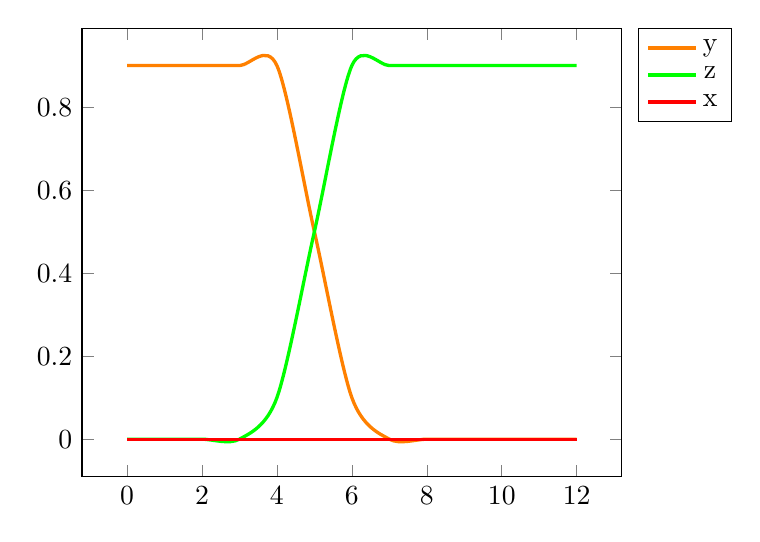
\begin{tikzpicture}
\begin{axis}[domain=0:1,legend pos=outer north east]
\addplot[orange,very thick][smooth]coordinates {(0,0.9)(1,0.9)(2,0.9)(3,0.9)(4,0.9)(5,0.5)(6,0.1)(7,0)(8,0)(9,0)(10,0)(11,0)(12,0)};
\addplot[green,very thick][smooth]coordinates {(0,0)(1,0)(2,0)(3,0)(4,0.1)(5,0.5)(6,0.9)(7,0.9)(8,0.9)(9,0.9)(10,0.9)(11,0.9)(12,0.9)};
\addplot[red,very thick]coordinates {(0,0)(12,0)};

\legend{y,z,x}

\end{axis}
\end{tikzpicture}
\end{adjustbox}
\fi %Something like uncommenting (END)

\begin{figure}
	\centering
	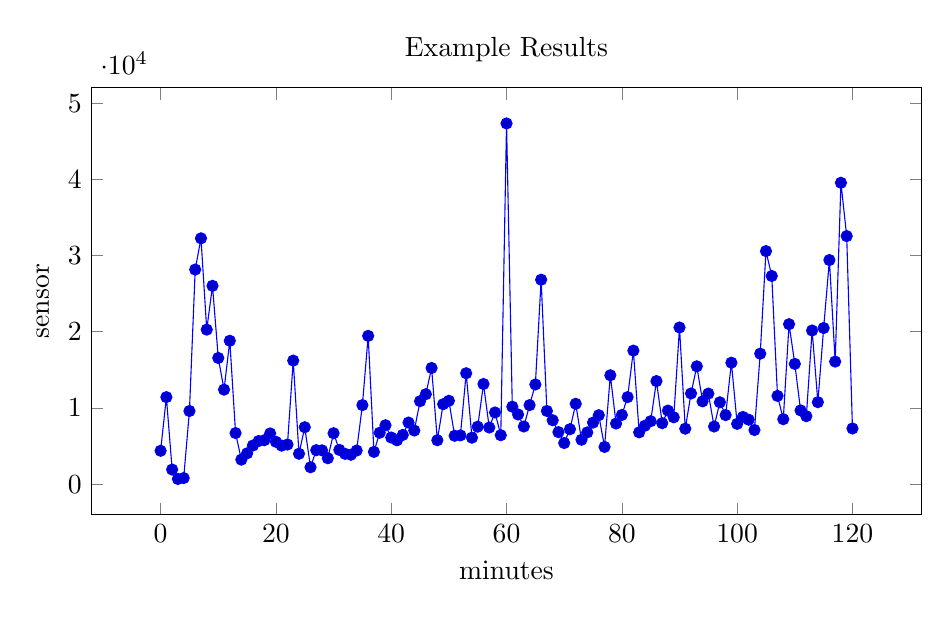
\begin{tikzpicture}
\begin{axis}[
	height=7cm,
	width=\textwidth,
	xlabel=minutes,
	ylabel=sensor,
	title=Example Results,
	unbounded coords=discard],
	
	\addplot coordinates {
(0 , 4383.0)
(1 , 11423.0)
(2 , 1918.0)
(3 , 684.0)
(4 , 805.0)
(5 , 9602.0)
(6 , 28165.0)
(7 , 32264.0)
(8 , 20283.0)
(9 , 26030.0)
(10 , 16563.0)
(11 , 12407.0)
(12 , 18819.0)
(13 , 6708.0)
(14 , 3220.0)
(15 , 4047.0)
(16 , 5069.0)
(17 , 5662.0)
(18 , 5772.0)
(19 , 6661.0)
(20 , 5561.0)
(21 , 5056.0)
(22 , 5205.0)
(23 , 16217.0)
(24 , 3994.0)
(25 , 7474.0)
(26 , 2220.0)
(27 , 4465.0)
(28 , 4437.0)
(29 , 3405.0)
(30 , 6689.0)
(31 , 4498.0)
(32 , 3983.0)
(33 , 3864.0)
(34 , 4413.0)
(35 , 10377.0)
(36 , 19460.0)
(37 , 4237.0)
(38 , 6751.0)
(39 , 7734.0)
(40 , 6122.0)
(41 , 5758.0)
(42 , 6460.0)
(43 , 8085.0)
(44 , 7039.0)
(45 , 10894.0)
(46 , 11810.0)
(47 , 15247.0)
(48 , 5769.0)
(49 , 10496.0)
(50 , 10942.0)
(51 , 6352.0)
(52 , 6403.0)
(53 , 14557.0)
(54 , 6105.0)
(55 , 7545.0)
(56 , 13146.0)
(57 , 7435.0)
(58 , 9412.0)
(59 , 6426.0)
(60 , 47340.0)
(61 , 10167.0)
(62 , 9147.0)
(63 , 7569.0)
(64 , 10373.0)
(65 , 13084.0)
(66 , 26832.0)
(67 , 9606.0)
(68 , 8393.0)
(69 , 6832.0)
(70 , 5402.0)
(71 , 7218.0)
(72 , 10548.0)
(73 , 5827.0)
(74 , 6796.0)
(75 , 8080.0)
(76 , 9051.0)
(77 , 4888.0)
(78 , 14292.0)
(79 , 7959.0)
(80 , 9081.0)
(81 , 11426.0)
(82 , 17525.0)
(83 , 6801.0)
(84 , 7673.0)
(85 , 8264.0)
(86 , 13528.0)
(87 , 8007.0)
(88 , 9657.0)
(89 , 8775.0)
(90 , 20563.0)
(91 , 7282.0)
(92 , 11904.0)
(93 , 15465.0)
(94 , 10871.0)
(95 , 11887.0)
(96 , 7567.0)
(97 , 10745.0)
(98 , 9067.0)
(99 , 15943.0)
(100 , 7914.0)
(101 , 8823.0)
(102 , 8461.0)
(103 , 7110.0)
(104 , 17129.0)
(105 , 30584.0)
(106 , 27321.0)
(107 , 11586.0)
(108 , 8531.0)
(109 , 20998.0)
(110 , 15785.0)
(111 , 9681.0)
(112 , 8923.0)
(113 , 20168.0)
(114 , 10760.0)
(115 , 20493.0)
(116 , 29414.0)
(117 , 16085.0)
(118 , 39551.0)
(119 , 32556.0)
(120 , 7311.0)
};


\end{axis}
\end{tikzpicture}
 	\vspace{10 mm}
\end{figure}


\chapter{Conclusions}

And a fancy conclusion...


\section{Future Work}
The results give evidence that it is very hard to find general patterns in the influences in the cognitive performance. The individual results were more clear but just valid for a single person. 
In my opinion it would be a good idea to let people individually gather data about their environment and working patterns continuously. A machine learning algorithm on the phone could find correlations between the individual performance and the data. Also, as the first experiment was just focusing on one single task, it would make sense to send the gathered data of each user to a Server that is analyzing it in relation to the data sets of the other participants. 
In experiment one, some information from some participants were not gathered because of the permissions and settings of their individual mobile devices or in some cases probably even missing sensors that were not built in that device. 
Therefore, to be able to eliminate the hardware issues a custom device to place on the desk would help to avoid these issues. It would also allow to add more sensors such as temperature, humidity etc. and with the same hardware guarantee that the sensors are working equally. 

%\addcontentsline {toc}{chapter}{Appendices}       %% Force Appendices to appear in contents
\begin{appendix}
\chapter{Abbreviations}




\begin{tabular}{p{40mm}|p{100mm}}
	\textbf{Short Term}&\textbf{Expanded Term}\\
	\hline
	LOC		&	Lines of Code\\
	KLOC	&	Thousand lines of code\\
	PSP		& 	Personal Software Process\\
	CSS 		& Cascading Style Sheets\\
	HTML 	& HyperText Markup Language\\
	GUI		& Graphical User Interface\\
	UI			& User Interface\\
	UX 		& User Experience\\
	SHA 		& Secure Hash Algorithm\\
	AES		& Advanced Encryption Standard\\
	RSA		& Rivest-Shamir-Adleman\\
	CBC 		& Cipher Block Chaining\\
	PKCS 	& Public Key Cryptography Standards\\
	SMS 		& Short Message Service\\
	API		& Application programming interface\\
	APK		& Android application package\\
\end{tabular}
\chapter{Source Code}


\begin{itemize}
\item Android Application for gathering the data
\subitem \url{https://github.com/MiChrFri/}

\item Java Application for decrypting the data
\subitem \url{https://github.com/MiChrFri/}

\item Python toolset for formatting the results
\subitem \url{https://github.com/MiChrFri/AnnaLize}

\item Website and Backend
\subitem \url{https://github.com/MiChrFri/}

\end{itemize}

\chapter{Participant data}

These are the results of the measurements from Experiment one for each participant. 

\newpage
\section{Participant 1}

\subsection{date \& time}
\begin{table}[ht]
  \begin{tabular}{|P{3cm}|P{3cm}|}
	\multicolumn{2}{c}{\textbf{2016-08-03}}    	\\ \hline
    Start Time      			& End Time   					\\ \hline
   \textbf{15:38:54} 	& \textbf{15:56:12}    	\\ \hline
   \multicolumn{2}{c}{Duration}    						\\ \hline
   \multicolumn{2}{c}{\textbf{00:17:18}} 			\\ \hline
  \end{tabular}
  \newline\newline
  \caption{p1: date and time}\label{dandt1}
\end{table}

\subsection{Questions}
\begin{itemize}
  \item[\Checkmark] Are you a Student?
  \item[\XSolidBrush] Did you work in a team?
  \item[\XSolidBrush] Did you listen to music?
  \item[\Checkmark] Did you feel tired?
  \item[\XSolidBrush] Did you enjoy the tasks?
  \item[\XSolidBrush] Did you give all you attention to the tasks?
  \item[\XSolidBrush] Were you distracted during the tasks?
  \item[\Checkmark] Did you feel stressed
  \item[\XSolidBrush] Do you think the tasks were easy?  
\end{itemize}

\newpage

\subsection{Accelerometer}
\begin{figure}[ht]
	\centering
	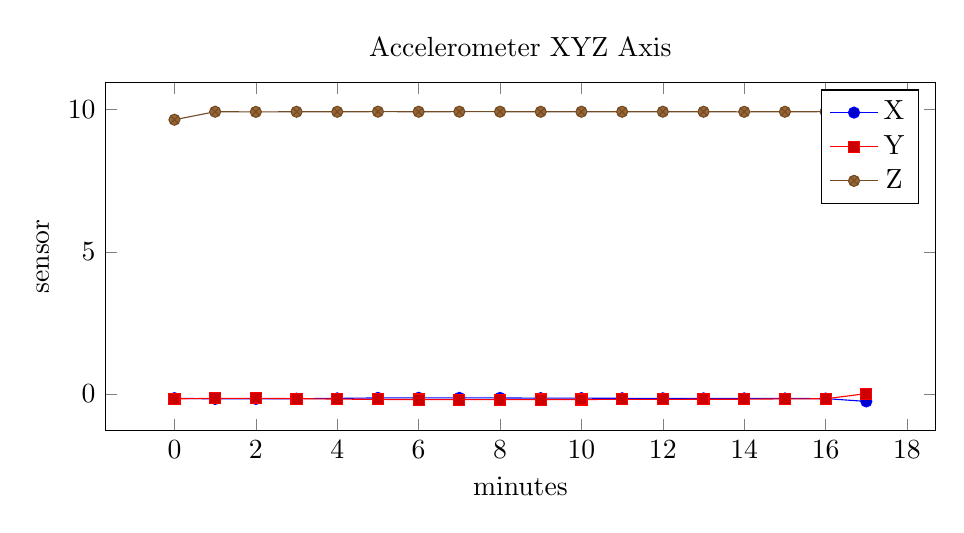
\begin{tikzpicture}
\begin{axis}[
	height=6cm,
	width=\textwidth,
	xlabel=minutes,
	ylabel=sensor,
	title=Accelerometer XYZ Axis,
	unbounded coords=discard],
	
%X
\addplot coordinates {
(0 , -0.144712392571)
(1 , -0.171607927941)
(2 , -0.170622079706)
(3 , -0.162515509394)
(4 , -0.151926182059)
(5 , -0.135589277353)
(6 , -0.132913407353)
(7 , -0.134673849412)
(8 , -0.135671431818)
(9 , -0.144321071176)
(10 , -0.143968983235)
(11 , -0.149250311471)
(12 , -0.150024906176)
(13 , -0.152322015758)
(14 , -0.152559941765)
(15 , -0.156679375)
(16 , -0.158615859706)
(17 , -0.258813207)
};

%Y
\addplot coordinates {
(0 , -0.17022774)
(1 , -0.149285518824)
(2 , -0.151151587353)
(3 , -0.160048757273)
(4 , -0.176325913529)
(5 , -0.187980040294)
(6 , -0.193965545882)
(7 , -0.195585153235)
(8 , -0.195780402121)
(9 , -0.193296577941)
(10 , -0.191571342647)
(11 , -0.185761882941)
(12 , -0.185902718235)
(13 , -0.183047602727)
(14 , -0.180586184118)
(15 , -0.168051834118)
(16 , -0.165798468824)
(17 , 0.01532289)
};

%Z
\addplot coordinates {
(0 , 9.64186077143)
(1 , 9.9233675)
(2 , 9.91780444118)
(3 , 9.92204354545)
(4 , 9.92065644118)
(5 , 9.92477579412)
(6 , 9.92287461765)
(7 , 9.92414205882)
(8 , 9.92422)
(9 , 9.92181826471)
(10 , 9.92354352941)
(11 , 9.92209991176)
(12 , 9.92389579412)
(13 , 9.92153551515)
(14 , 9.91977617647)
(15 , 9.92181838235)
(16 , 9.92442373529)
(17 , 9.9312684)
};

\addlegendentry{X}
\addlegendentry{Y}
\addlegendentry{Z}
\end{axis}
\end{tikzpicture}
	\vspace{5 mm}
\end{figure}

\FloatBarrier

\subsection{Light}
\begin{figure}[ht]
	\centering
	\begin{tikzpicture}
\begin{axis}[
	height=6cm,
	width=\textwidth,
	xlabel=minutes,
	ylabel=sensor,
	title=Light,
	unbounded coords=discard],
	
\addplot coordinates {
(0 , 0.0)
(1 , 0.0)
(2 , 0.0)
(3 , 0.0)
(4 , 0.0)
(5 , 0.0)
(6 , 0.0)
(7 , 0.0)
(8 , 0.0)
(9 , 0.0)
(10 , 0.0)
(11 , 0.0)
(12 , 0.0)
(13 , 0.0)
(14 , 0.0)
(15 , 0.0)
(16 , 0.0)
(17 , 0.0)
};

\end{axis}
\end{tikzpicture}
	\vspace{5 mm}
\end{figure}

\newpage
\FloatBarrier

\subsection{Volume}
\begin{figure}[ht]
	\centering
	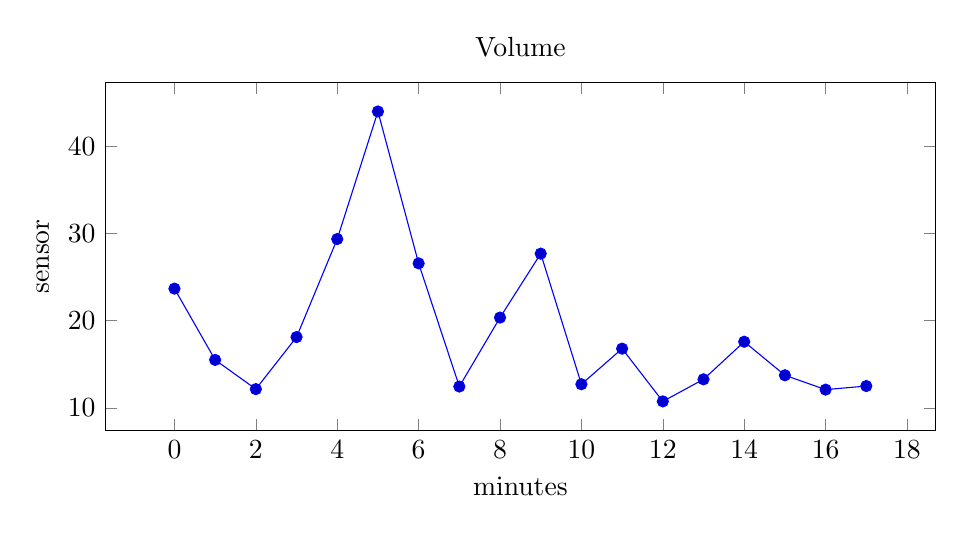
\begin{tikzpicture}
\begin{axis}[
	height=6cm,
	width=\textwidth,
	xlabel=minutes,
	ylabel=sensor,
	title=Volume,
	unbounded coords=discard],

\addplot coordinates {
(0 , 23.6857142857)
(1 , 15.5)
(2 , 12.1470588235)
(3 , 18.1212121212)
(4 , 29.3823529412)
(5 , 44.0294117647)
(6 , 26.5882352941)
(7 , 12.4411764706)
(8 , 20.3636363636)
(9 , 27.7058823529)
(10 , 12.7058823529)
(11 , 16.7941176471)
(12 , 10.7352941176)
(13 , 13.2727272727)
(14 , 17.5882352941)
(15 , 13.7352941176)
(16 , 12.0882352941)
(17 , 12.5)
};

\end{axis}
\end{tikzpicture}
 	\vspace{5 mm}
\end{figure}

\FloatBarrier

\subsection{Location}
No data gathered
\newpage
\section{Participant 2}

% JC

\subsection{Date \& Time}
\begin{table}[ht]
  \begin{tabular}{|P{3cm}|P{3cm}|}
	\multicolumn{2}{c}{\textbf{2016-08-03}}    	\\ \hline
    Start Time      			& End Time   					\\ \hline
   \textbf{12:23:50} 	& \textbf{12:42:23}    	\\ \hline
   \multicolumn{2}{c}{Duration}    						\\ \hline
   \multicolumn{2}{c}{\textbf{00:18:33}} 			\\ \hline
  \end{tabular}
  \newline\newline
  \caption{P2: Date and Time}\label{dandt2}
\end{table}

\subsection{Questions}
\begin{itemize} 
  \item[\XSolidBrush] Are you a Student?
  \item[\Checkmark] Did you work in a team?
  \item[\Checkmark] Did you listen to music?
  \item[\XSolidBrush] Did you feel tired?
  \item[\Checkmark] Did you enjoy the tasks?
  \item[\Checkmark] Did you give all you attention to the tasks?
  \item[\XSolidBrush] Were you distracted during the tasks?
  \item[\XSolidBrush] Did you feel stressed
  \item[\Checkmark] Do you think the tasks were easy?  
\end{itemize}


\FloatBarrier
\newpage
\subsection{Accelerometer}

\begin{figure}[ht]
	\centering
	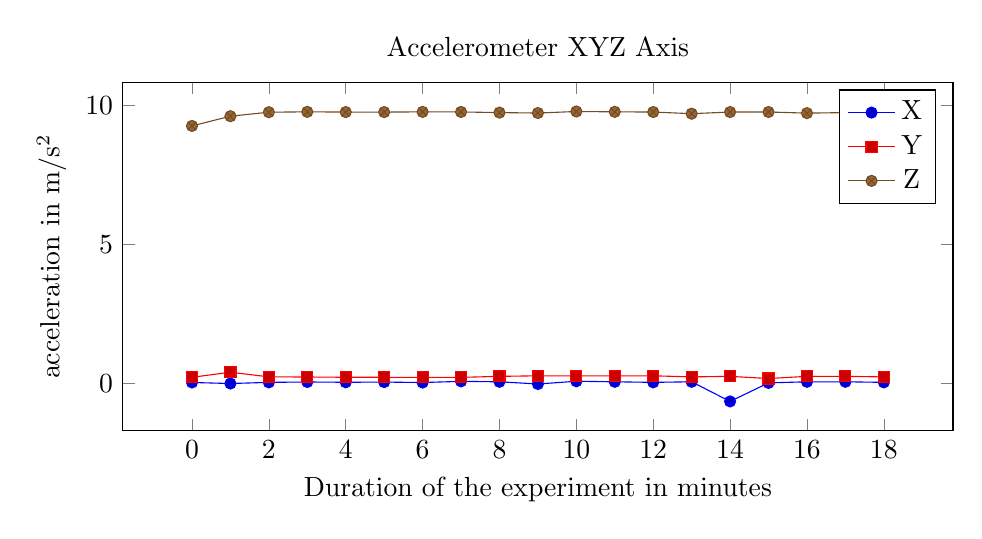
\begin{tikzpicture}
\begin{axis}[
	height=6cm,
	width=\textwidth,
	xlabel=Duration of the experiment in minutes,
	ylabel=acceleration in m/s$^2$,
	title=Accelerometer XYZ Axis,
	unbounded coords=discard],
	
%X
\addplot coordinates {
(0 , 0.0349651822609)
(1 , -0.00309673126316)
(2 , 0.0382930208571)
(3 , 0.0523034957619)
(4 , 0.0420292439048)
(5 , 0.049033425)
(6 , 0.0326879590952)
(7 , 0.0751864109167)
(8 , 0.05883789)
(9 , -0.019607544)
(10 , 0.07846069)
(11 , 0.05883789)
(12 , 0.039230347)
(13 , 0.05883789)
(14 , -0.64723206)
(15 , 0.019607544)
(16 , 0.05883789)
(17 , 0.05883789)
(18 , 0.039230347)
};

%Y
\addplot coordinates {
(0 , 0.220863674783)
(1 , 0.403620667895)
(2 , 0.23722984381)
(3 , 0.231626238095)
(4 , 0.222285678571)
(5 , 0.221095690909)
(6 , 0.217615762857)
(7 , 0.219015755833)
(8 , 0.25497437)
(9 , 0.2745819)
(10 , 0.2745819)
(11 , 0.2745819)
(12 , 0.2745819)
(13 , 0.23536682)
(14 , 0.25497437)
(15 , 0.17651367)
(16 , 0.25497437)
(17 , 0.25497437)
(18 , 0.23536682)
};

%Z
\addplot coordinates {
(0 , 9.26770895652)
(1 , 9.61774347368)
(2 , 9.76181833333)
(3 , 9.77489447619)
(4 , 9.76648904762)
(5 , 9.76563831818)
(6 , 9.77396304762)
(7 , 9.77069233333)
(8 , 9.74780316161)
(9 , 9.73178425312)
(10 , 9.78743477033)
(11 , 9.77489304762)
(12 , 9.76742633556)
(13 , 9.70858834222)
(14 , 9.76742655645)
(15 , 9.76935722354)
(16 , 9.72819595862)
(17 , 9.74780318532)
(18 , 9.70858858813)
};

\addlegendentry{X}
\addlegendentry{Y}
\addlegendentry{Z}
\end{axis}
\end{tikzpicture}
 	\vspace{5 mm}
\end{figure}

\FloatBarrier
\subsection{Light Level}
\begin{figure}[ht]
	\centering
	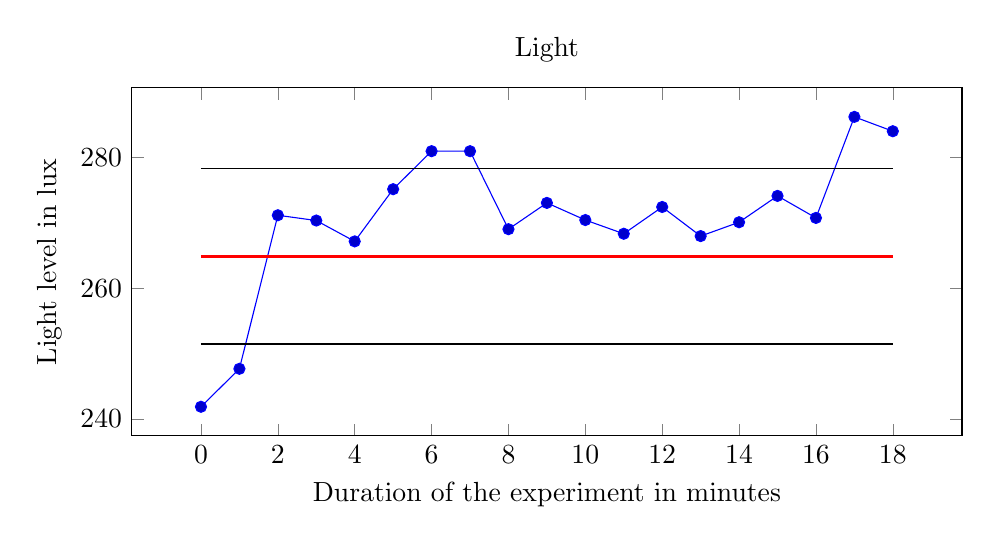
\begin{tikzpicture}
\begin{axis}[
	height=6cm,
	width=\textwidth,
	xlabel=Duration of the experiment in minutes,
	ylabel=Light level in lux,
	title=Light,
	unbounded coords=discard],
	
\addplot coordinates {
(0 , 241.869565217)
(1 , 247.684210526)
(2 , 271.19047619)
(3 , 270.380952381)
(4 , 267.19047619)
(5 , 275.181818182)
(6 , 281.0)
(7 , 281.0)
(8 , 269.056565454)
(9 , 273.082245)
(10 , 270.457685359)
(11 , 268.358045125)
(12 , 272.456782138)
(13 , 268.0)
(14 , 270.121246868)
(15 , 274.154865478)
(16 , 270.782398425)
(17 , 286.252546845)
(18 , 284.054086785)
};

\addplot[mark=none, red, very thick] coordinates {(0, 264.928214098) (18, 264.928214098)};

\addplot[mark=none, black] coordinates {(0, 251.47691699) (18, 251.47691699)};
\addplot[mark=none, black] coordinates {(0, 278.379511206) (18, 278.379511206)};

\end{axis}
\end{tikzpicture}
 	\vspace{5 mm}
\end{figure}

\newpage
\FloatBarrier
\newpage
\subsection{Noise Level}
\begin{figure}[ht]
	\centering
	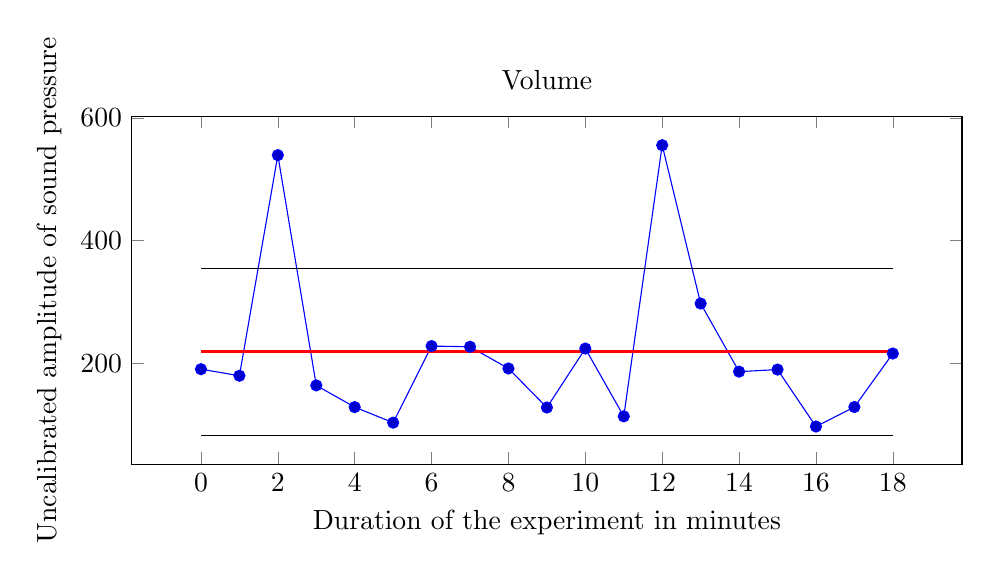
\begin{tikzpicture}
\begin{axis}[
	height=6cm,
	width=\textwidth,
	ylabel=Uncalibrated amplitude of sound pressure,
	xlabel=Duration of the experiment in minutes,
	title=Volume,
	unbounded coords=discard],

\addplot coordinates {
(0 , 190.434782609)
(1 , 179.736842105)
(2 , 539.238095238)
(3 , 164.0)
(4 , 128.619047619)
(5 , 103.318181818)
(6 , 228.095238095)
(7 , 227.0)
(8 , 191.596186522)
(9 , 127.958334583)
(10 , 224.056548712)
(11 , 113.580190875)
(12 , 555.4568753253)
(13 , 297.4565454254)
(14 , 186.4298341674)
(15 , 189.8012096456)
(16 , 97.0)
(17 , 128.8121400108)
(18 , 215.9958225684)
};

\addplot[mark=none, red, very thick] coordinates {(0, 219.063169641) (18, 219.063169641)};

\addplot[mark=none, black] coordinates {(0, 83.0123913636) (18, 83.0123913636)};
\addplot[mark=none, black] coordinates {(0, 355.113947918) (18, 355.113947918)};

\end{axis}
\end{tikzpicture}
 	\vspace{5 mm}
\end{figure}

\FloatBarrier

\subsection{Location}
minute 0 : -3.6881917, 40.4579957
minute 1 : -3.68815341053, 40.4579801474)
from minute 2 : -3.6881432, 40.457976)

Madrid, Spain 

\FloatBarrier
\newpage
\section{Participant 3}

\subsection{date \& time}
\begin{table}[ht]
  \begin{tabular}{|P{3cm}|P{3cm}|}
	\multicolumn{2}{c}{\textbf{2016-07-28}}    	\\ \hline
    Start Time      			& End Time   					\\ \hline
   \textbf{12:52:44} 	& \textbf{13:04:45}    	\\ \hline
   \multicolumn{2}{c}{Duration}    						\\ \hline
   \multicolumn{2}{c}{\textbf{00:12:01}} 			\\ \hline
  \end{tabular}
  \newline\newline
 \caption{p3: date and time}\label{dandt1}
\end{table}

\subsection{Questions}
\begin{itemize} 
  \item[\Checkmark] Are you a Student?
  \item[\XSolidBrush] Did you work in a team?
  \item[\Checkmark] Did you listen to music?
  \item[\XSolidBrush] Did you feel tired?
  \item[\Checkmark] Did you enjoy the tasks?
  \item[\Checkmark] Did you give all you attention to the tasks?
  \item[\XSolidBrush] Were you distracted during the tasks?
  \item[\XSolidBrush] Did you feel stressed
  \item[\XSolidBrush] Do you think the tasks were easy?  
\end{itemize}


\FloatBarrier
\newpage
\subsection{Accelerometer}

\begin{figure}[ht]
	\centering
	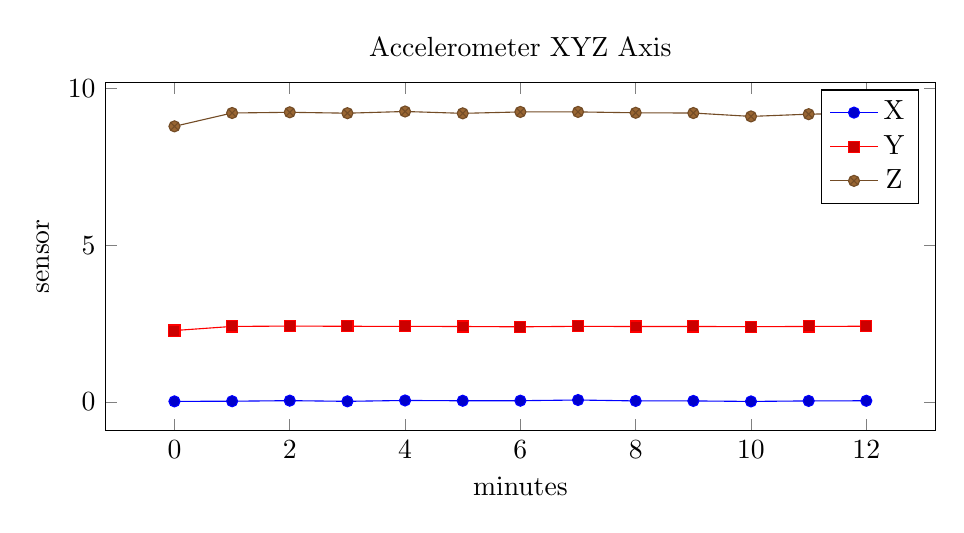
\begin{tikzpicture}
\begin{axis}[
	height=6cm,
	width=\textwidth,
	xlabel=minutes,
	ylabel=sensor,
	title=Accelerometer XYZ Axis,
	unbounded coords=discard],
	
%X
\addplot coordinates {
(0 , 0.019438637881)
(1 , 0.0247400849444)
(2 , 0.0424115735714)
(3 , 0.02101577)
(4 , 0.0486535994286)
(5 , 0.0389057787143)
(6 , 0.041366485)
(7 , 0.0629475533333)
(8 , 0.034117374125)
(9 , 0.033618582)
(10 , 0.0179565136667)
(11 , 0.0341173747143)
(12 , 0.038905777)
};

%Y
\addplot coordinates {
(0 , 2.2777979)
(1 , 2.40836742222)
(2 , 2.42019587143)
(3 , 2.41288974444)
(4 , 2.41164518571)
(5 , 2.40600168571)
(6 , 2.39666241111)
(7 , 2.4114599)
(8 , 2.4058734375)
(9 , 2.40826766667)
(10 , 2.3990899)
(11 , 2.40848141429)
(12 , 2.4145525)
};

%Z
\addplot coordinates {
(0 , 8.7865777619)
(1 , 9.21202333333)
(2 , 9.234265)
(3 , 9.20590511111)
(4 , 9.26008828571)
(5 , 9.20108792857)
(6 , 9.24580855556)
(7 , 9.24680616667)
(8 , 9.2185745)
(9 , 9.21099291667)
(10 , 9.1032535)
(11 , 9.17449528571)
(12 , 9.20391)
};

\addlegendentry{X}
\addlegendentry{Y}
\addlegendentry{Z}
\end{axis}
\end{tikzpicture}
 	\vspace{5 mm}
\end{figure}

\FloatBarrier
\subsection{Light}
\begin{figure}[ht]
	\centering
	\begin{tikzpicture}
\begin{axis}[
	height=6cm,
	width=\textwidth,
	xlabel=minutes,
	ylabel=sensor,
	title=Light,
	unbounded coords=discard],
	
\addplot coordinates {
(0 , 330.986057143)
(1 , 327.141866667)
(2 , 324.539771429)
(3 , 322.701066667)
(4 , 329.208342857)
(5 , 335.669942857)
(6 , 346.047466667)
(7 , 352.541066667)
(8 , 368.9453)
(9 , 374.263066667)
(10 , 355.196133333)
(11 , 340.515885714)
(12 , 332.4064)
};

\end{axis}
\end{tikzpicture}
 	\vspace{5 mm}
\end{figure}

\newpage
\FloatBarrier
\newpage
\subsection{Volume}
\begin{figure}[ht]
	\centering
	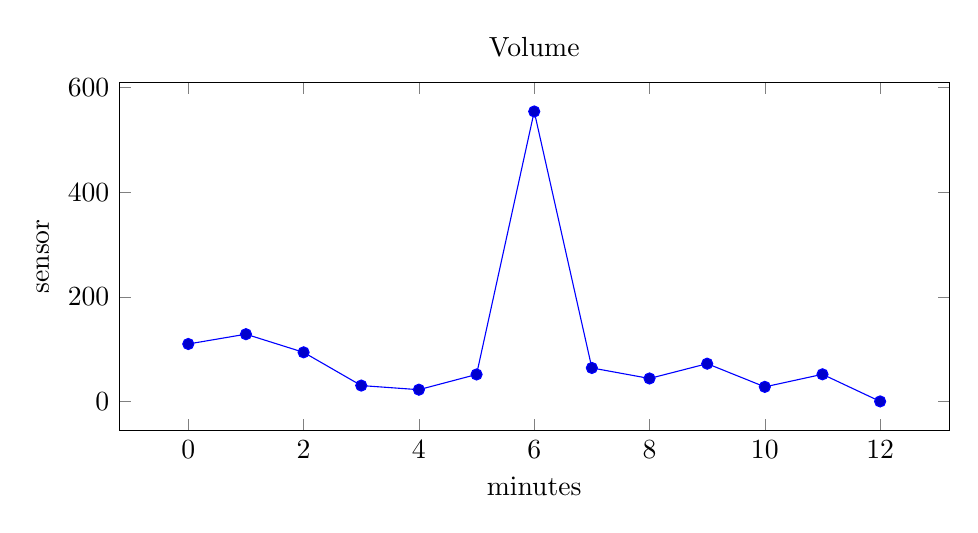
\begin{tikzpicture}
\begin{axis}[
	height=6cm,
	width=\textwidth,
	xlabel=minutes,
	ylabel=sensor,
	title=Volume,
	unbounded coords=discard],

\addplot coordinates {
(0 , 109.80952381)
(1 , 128.555555556)
(2 , 93.8571428571)
(3 , 30.3333333333)
(4 , 22.4285714286)
(5 , 51.5714285714)
(6 , 554.333333333)
(7 , 64.0)
(8 , 43.875)
(9 , 72.1666666667)
(10 , 27.8333333333)
(11 , 51.8571428571)
(12 , 0.0)
};

\end{axis}
\end{tikzpicture}
 	\vspace{5 mm}
\end{figure}

\FloatBarrier
\subsection{Steps}
\begin{figure}[ht]
	\centering
	\begin{tikzpicture}
\begin{axis}[
	height=6cm,
	width=\textwidth,
	xlabel=minutes,
	ylabel=sensor,
	title=Steps,
	unbounded coords=discard],

\addplot coordinates {
(0 , 0.0)
(1 , 0.0)
(2 , 0.0)
(3 , 0.0)
(4 , 0.0)
(5 , 0.0)
(6 , 0.0)
(7 , 0.0)
(8 , 0.0)
(9 , 0.0)
(10 , 0.0)
(11 , 0.0)
(12 , 0.0)
};

\end{axis}
\end{tikzpicture}
 	\vspace{5 mm}
\end{figure}

\newpage
\FloatBarrier

\subsection{Location}
No data gathered

\FloatBarrier
\subsection{Weather}
No data gathered

\FloatBarrier
\newpage
\section{Participant 4}

%% MK

\subsection{Date \& Time}
\begin{table}[ht]
  \begin{tabular}{|P{3cm}|P{3cm}|}
	\multicolumn{2}{c}{\textbf{2016-08-04}}    	\\ \hline
    Start Time      			& End Time   					\\ \hline
   \textbf{10:20:13} 	& \textbf{11:20:41}    	\\ \hline
   \multicolumn{2}{c}{Duration}    						\\ \hline
   \multicolumn{2}{c}{\textbf{01:00:28}} 			\\ \hline
  \end{tabular}
  \newline\newline
  \caption{P4: Date and Time}\label{dandt4}
\end{table}

\subsection{Questions}
\begin{itemize} 
  \item[\Checkmark] Are you a Student?
  \item[\XSolidBrush] Did you work in a team?
  \item[\XSolidBrush] Did you listen to music?
  \item[\Checkmark] Did you feel tired?
  \item[\Checkmark] Did you enjoy the tasks?
  \item[\XSolidBrush] Did you give all you attention to the tasks?
  \item[\Checkmark] Were you distracted during the tasks?
  \item[\Checkmark] Did you feel stressed
  \item[\XSolidBrush] Do you think the tasks were easy?  
\end{itemize}


\FloatBarrier
\newpage

\subsection{Accelerometer}

\begin{figure}[ht]
	\centering
	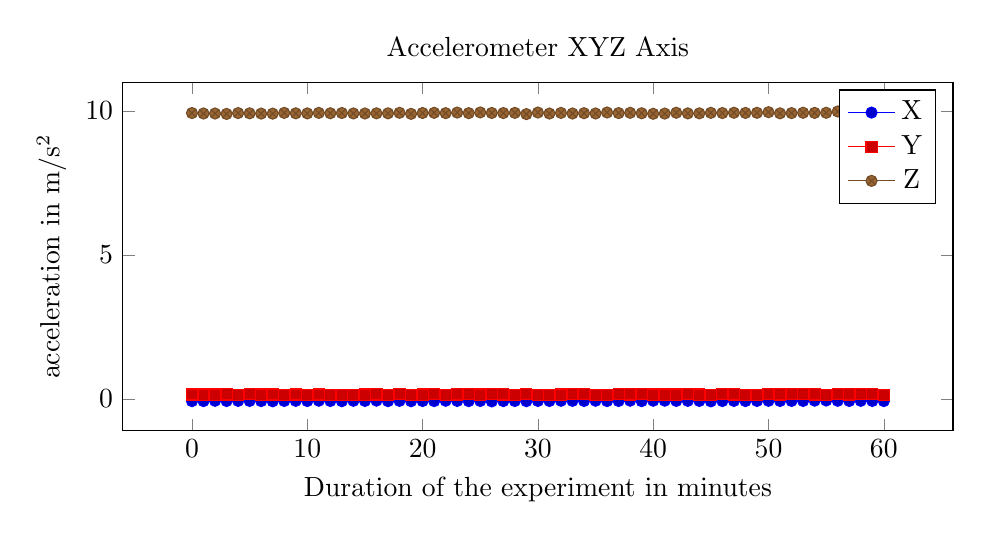
\begin{tikzpicture}
\begin{axis}[
	height=6cm,
	width=\textwidth,
	xlabel=Duration of the experiment in minutes,
	ylabel=acceleration in m/s$^2$,
	title=Accelerometer XYZ Axis,
	unbounded coords=discard],
	
%X
\addplot coordinates {
(0 , -0.0747131762353)
(1 , -0.073247608625)
(2 , -0.063521163625)
(3 , -0.070778586)
(4 , -0.06584054825)
(5 , -0.0672371646667)
(6 , -0.0736217)
(7 , -0.0798067233333)
(8 , -0.0686337833333)
(9 , -0.06434417)
(10 , -0.07122749975)
(11 , -0.0600545593333)
(12 , -0.069282211)
(13 , -0.07631518)
(14 , -0.06299743325)
(15 , -0.0679354745)
(16 , -0.0568622886667)
(17 , -0.07481880275)
(18 , -0.064643445)
(19 , -0.0770134866667)
(20 , -0.0708284676667)
(21 , -0.0723048914)
(22 , -0.061451177)
(23 , -0.0666386146667)
(24 , -0.0737214611667)
(25 , -0.06823475)
(26 , -0.0831985105)
(27 , -0.073621705)
(28 , -0.0700303985)
(29 , -0.07571663)
(30 , -0.06808510825)
(31 , -0.0690328133333)
(32 , -0.06269815775)
(33 , -0.064942722)
(34 , -0.06853402325)
(35 , -0.061052144)
(36 , -0.0724246025)
(37 , -0.0694318475)
(38 , -0.05865794)
(39 , -0.074699092)
(40 , -0.060752869)
(41 , -0.0587576993333)
(42 , -0.066638614)
(43 , -0.065241995)
(44 , -0.0673369215)
(45 , -0.082001406)
(46 , -0.071526772)
(47 , -0.06688800775)
(48 , -0.072723875)
(49 , -0.067636197)
(50 , -0.06314707)
(51 , -0.06958148675)
(52 , -0.0672371633333)
(53 , -0.068035233)
(54 , -0.0580593925)
(55 , -0.0528434535714)
(56 , -0.06254852)
(57 , -0.0688017963684)
(58 , -0.06464344625)
(59 , -0.068234749)
(60 , -0.0725243588333)
};

%Y
\addplot coordinates {
(0 , 0.156256870588)
(1 , 0.15315409)
(2 , 0.15367782375)
(3 , 0.15786767)
(4 , 0.14454993)
(5 , 0.16360378)
(6 , 0.15382746)
(7 , 0.155822623333)
(8 , 0.145846786667)
(9 , 0.155323835)
(10 , 0.15083471)
(11 , 0.155822626667)
(12 , 0.1484405075)
(13 , 0.142455)
(14 , 0.144250655)
(15 , 0.15412673)
(16 , 0.157219246667)
(17 , 0.1415571775)
(18 , 0.160411515)
(19 , 0.147442923333)
(20 , 0.154226496667)
(21 , 0.159214414)
(22 , 0.148240986667)
(23 , 0.157219246667)
(24 , 0.161508855)
(25 , 0.154126735)
(26 , 0.165499195)
(27 , 0.15682021)
(28 , 0.15203181)
(29 , 0.187047005)
(30 , 0.143352825)
(31 , 0.15003664)
(32 , 0.1550245625)
(33 , 0.16011224)
(34 , 0.1593640525)
(35 , 0.15023616)
(36 , 0.14514848)
(37 , 0.16071079)
(38 , 0.15741876)
(39 , 0.162207164)
(40 , 0.15502456)
(41 , 0.15522408)
(42 , 0.153627943333)
(43 , 0.17238252)
(44 , 0.153528185)
(45 , 0.14584679)
(46 , 0.16190789)
(47 , 0.15816695)
(48 , 0.15263036)
(49 , 0.14754268)
(50 , 0.16011224)
(51 , 0.157269125)
(52 , 0.159812963333)
(53 , 0.165997983333)
(54 , 0.15831659)
(55 , 0.147499927143)
(56 , 0.172981075)
(57 , 0.157733788421)
(58 , 0.1634042675)
(59 , 0.1726818)
(60 , 0.140360076667)
};

%Z
\addplot coordinates {
(0 , 9.92474058824)
(1 , 9.9079546875)
(2 , 9.9084784375)
(3 , 9.89433775)
(4 , 9.923517)
(5 , 9.914589)
(6 , 9.905411)
(7 , 9.90421416667)
(8 , 9.93035066667)
(9 , 9.914988)
(10 , 9.91244375)
(11 , 9.930351)
(12 , 9.9172325)
(13 , 9.925762)
(14 , 9.9112465)
(15 , 9.9093015)
(16 , 9.914589)
(17 , 9.91423975)
(18 , 9.9332435)
(19 , 9.89643233333)
(20 , 9.92596133333)
(21 , 9.9329444)
(22 , 9.92097333333)
(23 , 9.940925)
(24 , 9.92167158333)
(25 , 9.9455135)
(26 , 9.9275575)
(27 , 9.92396633333)
(28 , 9.93055)
(29 , 9.8877535)
(30 , 9.94282025)
(31 , 9.907406)
(32 , 9.92965225)
(33 , 9.908703)
(34 , 9.919028)
(35 , 9.90940133333)
(36 , 9.9437185)
(37 , 9.923218)
(38 , 9.932944)
(39 , 9.9166634)
(40 , 9.8985275)
(41 , 9.90640833333)
(42 , 9.935538)
(43 , 9.9128925)
(44 , 9.91379075)
(45 , 9.931947)
(46 , 9.9242655)
(47 , 9.9341415)
(48 , 9.9284555)
(49 , 9.932645)
(50 , 9.954492)
(51 , 9.91409)
(52 , 9.92296833333)
(53 , 9.93414133333)
(54 , 9.930101)
(55 , 9.93345728571)
(56 , 9.9787335)
(57 , 9.92550976316)
(58 , 9.91049875)
(59 , 9.9203745)
(60 , 9.92167166667)
};

\addlegendentry{X}
\addlegendentry{Y}
\addlegendentry{Z}
\end{axis}
\end{tikzpicture}
 	\vspace{5 mm}
\end{figure}

\FloatBarrier
\subsection{Light Level}
\begin{figure}[ht]
	\centering
	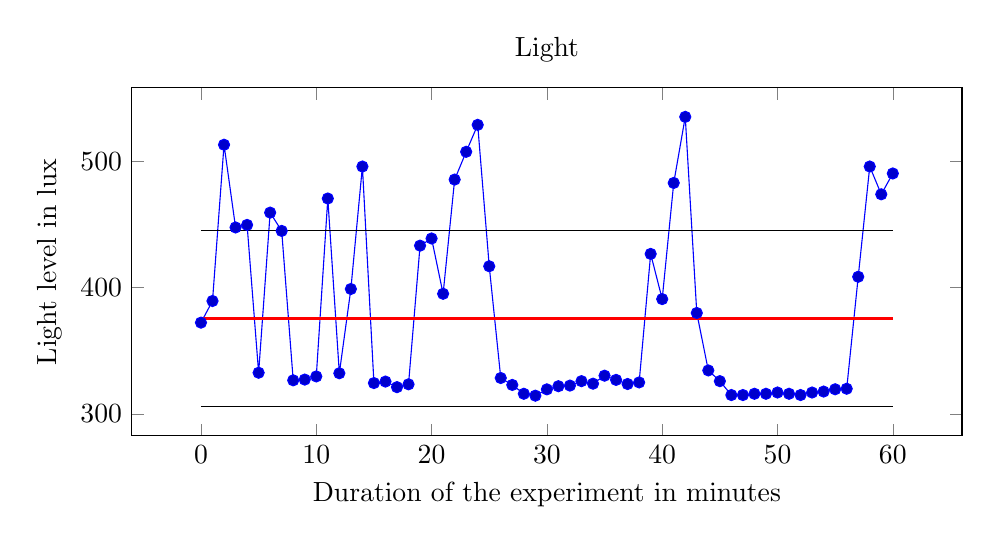
\begin{tikzpicture}
\begin{axis}[
	height=6cm,
	width=\textwidth,
	xlabel=Duration of the experiment in minutes,
	ylabel=Light level in lux,
	title=Light,
	unbounded coords=discard],
	
\addplot coordinates {
(0 , 372.352941176)
(1 , 389.5)
(2 , 513.25)
(3 , 447.75)
(4 , 449.75)
(5 , 332.666666667)
(6 , 459.5)
(7 , 445.0)
(8 , 326.666666667)
(9 , 327.25)
(10 , 329.75)
(11 , 470.666666667)
(12 , 332.25)
(13 , 399.0)
(14 , 496.0)
(15 , 324.5)
(16 , 325.666666667)
(17 , 321.25)
(18 , 323.5)
(19 , 433.333333333)
(20 , 439.0)
(21 , 395.2)
(22 , 485.666666667)
(23 , 507.666666667)
(24 , 529.0)
(25 , 417.0)
(26 , 328.5)
(27 , 323.0)
(28 , 316.0)
(29 , 314.5)
(30 , 319.5)
(31 , 322.0)
(32 , 322.5)
(33 , 326.0)
(34 , 324.0)
(35 , 330.333333333)
(36 , 327.0)
(37 , 323.75)
(38 , 325.0)
(39 , 426.8)
(40 , 391.0)
(41 , 483.0)
(42 , 535.333333333)
(43 , 380.0)
(44 , 334.5)
(45 , 326.0)
(46 , 315.0)
(47 , 315.0)
(48 , 316.0)
(49 , 316.0)
(50 , 317.0)
(51 , 316.0)
(52 , 315.0)
(53 , 317.0)
(54 , 317.75)
(55 , 319.571428571)
(56 , 320.0)
(57 , 408.684210526)
(58 , 496.0)
(59 , 474.0)
(60 , 490.5)
};

\addplot[mark=none, red, very thick] coordinates {(0, 375.580976338) (60, 375.580976338)};

\addplot[mark=none, black] coordinates {(0, 305.697485999) (60, 305.697485999)};
\addplot[mark=none, black] coordinates {(0, 445.464466676) (60, 445.464466676)};


\end{axis}
\end{tikzpicture}
 	\vspace{5 mm}
\end{figure}

\newpage
\FloatBarrier
\newpage
\subsection{Noise Level}
\begin{figure}[ht]
	\centering
	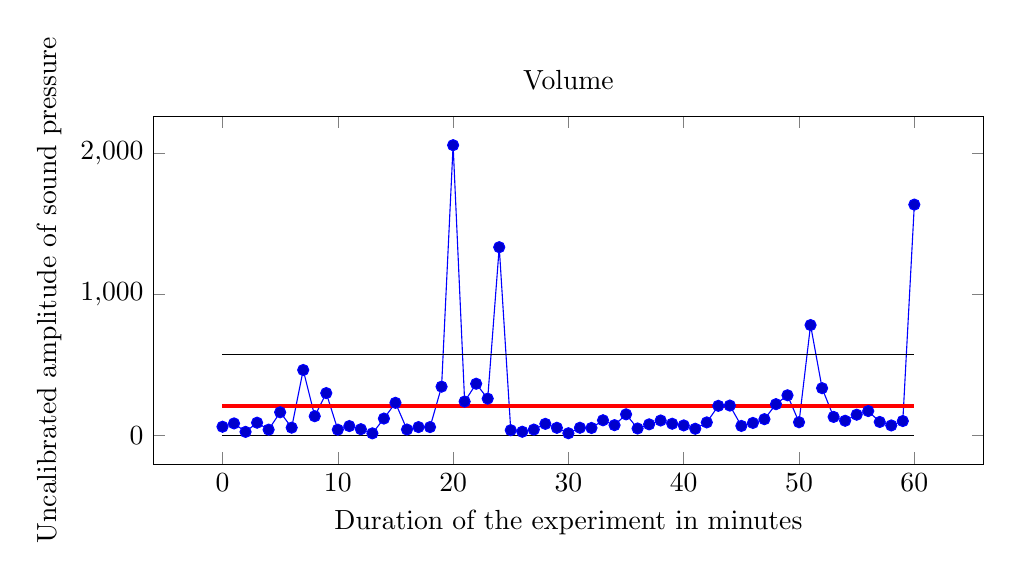
\begin{tikzpicture}
\begin{axis}[
	height=6cm,
	width=\textwidth,
	ylabel=Uncalibrated amplitude of sound pressure,
	xlabel=Duration of the experiment in minutes,
	title=Volume,
	unbounded coords=discard],

\addplot coordinates {
(0 , 59.5882352941)
(1 , 83.125)
(2 , 23.0)
(3 , 88.25)
(4 , 38.75)
(5 , 162.333333333)
(6 , 53.0)
(7 , 462.666666667)
(8 , 134.333333333)
(9 , 298.5)
(10 , 38.5)
(11 , 64.3333333333)
(12 , 42.0)
(13 , 12.5)
(14 , 117.75)
(15 , 229.5)
(16 , 39.6666666667)
(17 , 57.0)
(18 , 57.0)
(19 , 344.333333333)
(20 , 2060.0)
(21 , 238.6)
(22 , 365.0)
(23 , 259.0)
(24 , 1335.16666667)
(25 , 35.0)
(26 , 24.0)
(27 , 39.3333333333)
(28 , 80.0)
(29 , 52.0)
(30 , 13.25)
(31 , 52.3333333333)
(32 , 50.75)
(33 , 105.5)
(34 , 70.75)
(35 , 147.666666667)
(36 , 47.0)
(37 , 76.5)
(38 , 104.0)
(39 , 80.8)
(40 , 69.0)
(41 , 45.1666666667)
(42 , 90.3333333333)
(43 , 208.0)
(44 , 210.0)
(45 , 65.3333333333)
(46 , 86.5)
(47 , 113.25)
(48 , 220.0)
(49 , 283.0)
(50 , 91.5)
(51 , 782.0)
(52 , 333.666666667)
(53 , 129.333333333)
(54 , 102.0)
(55 , 145.0)
(56 , 171.0)
(57 , 93.5789473684)
(58 , 68.75)
(59 , 100.0)
(60 , 1637.83333333)
};

\addplot[mark=none, red, very thick] coordinates {(0, 208.000418295) (60, 208.000418295)};

\addplot[mark=none, black] coordinates {(0, 0) (60, 0)};
\addplot[mark=none, black] coordinates {(0, 571.657643466) (60, 571.657643466)};

\end{axis}
\end{tikzpicture}
 	\vspace{5 mm}
\end{figure}

\FloatBarrier

\subsection{Location}
53.3437734, -6.2510318

Dublin, Ireland 

\FloatBarrier
\chapter{Participant data}

These are the results of the measurements from Experiment one for each participant. 

\subsection{Graph descriptions}

\subsubsection{Accelerometer}
The accelerometer graph shows the changes of the three axis values over the time of the experiment. 

\subsubsection{Noise and Light}
The graphs of the noise and light level show the changes of the measurements (y-axis) over time (x-axis). 
The the thicker horizontal line indicates the average value and two lines, one below and the other one on top of the average is the range of the standard deviation and is treated different in the evaluation section.

\clearpage
\section{Participant 1}

\subsection{date \& time}
\begin{table}[ht]
  \begin{tabular}{|P{3cm}|P{3cm}|}
	\multicolumn{2}{c}{\textbf{2016-08-03}}    	\\ \hline
    Start Time      			& End Time   					\\ \hline
   \textbf{15:38:54} 	& \textbf{15:56:12}    	\\ \hline
   \multicolumn{2}{c}{Duration}    						\\ \hline
   \multicolumn{2}{c}{\textbf{00:17:18}} 			\\ \hline
  \end{tabular}
  \newline\newline
  \caption{p1: date and time}\label{dandt1}
\end{table}

\subsection{Questions}
\begin{itemize}
  \item[\Checkmark] Are you a Student?
  \item[\XSolidBrush] Did you work in a team?
  \item[\XSolidBrush] Did you listen to music?
  \item[\Checkmark] Did you feel tired?
  \item[\XSolidBrush] Did you enjoy the tasks?
  \item[\XSolidBrush] Did you give all you attention to the tasks?
  \item[\XSolidBrush] Were you distracted during the tasks?
  \item[\Checkmark] Did you feel stressed
  \item[\XSolidBrush] Do you think the tasks were easy?  
\end{itemize}

\newpage

\subsection{Accelerometer}
\begin{figure}[ht]
	\centering
	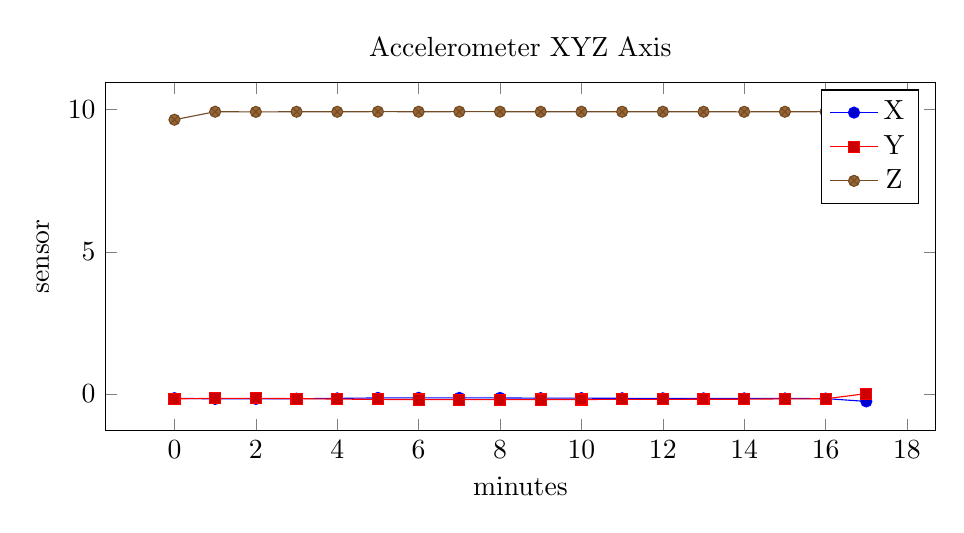
\begin{tikzpicture}
\begin{axis}[
	height=6cm,
	width=\textwidth,
	xlabel=minutes,
	ylabel=sensor,
	title=Accelerometer XYZ Axis,
	unbounded coords=discard],
	
%X
\addplot coordinates {
(0 , -0.144712392571)
(1 , -0.171607927941)
(2 , -0.170622079706)
(3 , -0.162515509394)
(4 , -0.151926182059)
(5 , -0.135589277353)
(6 , -0.132913407353)
(7 , -0.134673849412)
(8 , -0.135671431818)
(9 , -0.144321071176)
(10 , -0.143968983235)
(11 , -0.149250311471)
(12 , -0.150024906176)
(13 , -0.152322015758)
(14 , -0.152559941765)
(15 , -0.156679375)
(16 , -0.158615859706)
(17 , -0.258813207)
};

%Y
\addplot coordinates {
(0 , -0.17022774)
(1 , -0.149285518824)
(2 , -0.151151587353)
(3 , -0.160048757273)
(4 , -0.176325913529)
(5 , -0.187980040294)
(6 , -0.193965545882)
(7 , -0.195585153235)
(8 , -0.195780402121)
(9 , -0.193296577941)
(10 , -0.191571342647)
(11 , -0.185761882941)
(12 , -0.185902718235)
(13 , -0.183047602727)
(14 , -0.180586184118)
(15 , -0.168051834118)
(16 , -0.165798468824)
(17 , 0.01532289)
};

%Z
\addplot coordinates {
(0 , 9.64186077143)
(1 , 9.9233675)
(2 , 9.91780444118)
(3 , 9.92204354545)
(4 , 9.92065644118)
(5 , 9.92477579412)
(6 , 9.92287461765)
(7 , 9.92414205882)
(8 , 9.92422)
(9 , 9.92181826471)
(10 , 9.92354352941)
(11 , 9.92209991176)
(12 , 9.92389579412)
(13 , 9.92153551515)
(14 , 9.91977617647)
(15 , 9.92181838235)
(16 , 9.92442373529)
(17 , 9.9312684)
};

\addlegendentry{X}
\addlegendentry{Y}
\addlegendentry{Z}
\end{axis}
\end{tikzpicture}
	\vspace{5 mm}
\end{figure}

\FloatBarrier

\subsection{Light}
\begin{figure}[ht]
	\centering
	\begin{tikzpicture}
\begin{axis}[
	height=6cm,
	width=\textwidth,
	xlabel=minutes,
	ylabel=sensor,
	title=Light,
	unbounded coords=discard],
	
\addplot coordinates {
(0 , 0.0)
(1 , 0.0)
(2 , 0.0)
(3 , 0.0)
(4 , 0.0)
(5 , 0.0)
(6 , 0.0)
(7 , 0.0)
(8 , 0.0)
(9 , 0.0)
(10 , 0.0)
(11 , 0.0)
(12 , 0.0)
(13 , 0.0)
(14 , 0.0)
(15 , 0.0)
(16 , 0.0)
(17 , 0.0)
};

\end{axis}
\end{tikzpicture}
	\vspace{5 mm}
\end{figure}

\newpage
\FloatBarrier

\subsection{Volume}
\begin{figure}[ht]
	\centering
	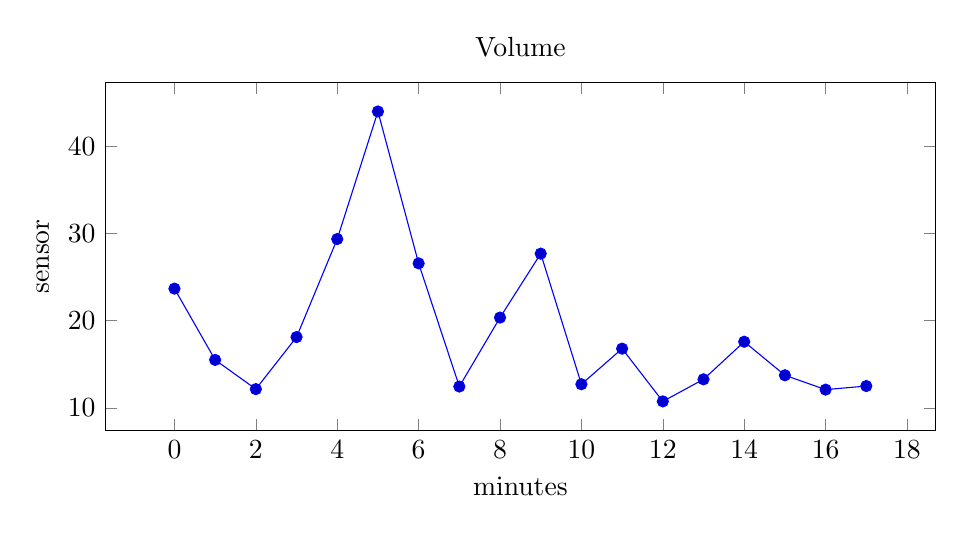
\begin{tikzpicture}
\begin{axis}[
	height=6cm,
	width=\textwidth,
	xlabel=minutes,
	ylabel=sensor,
	title=Volume,
	unbounded coords=discard],

\addplot coordinates {
(0 , 23.6857142857)
(1 , 15.5)
(2 , 12.1470588235)
(3 , 18.1212121212)
(4 , 29.3823529412)
(5 , 44.0294117647)
(6 , 26.5882352941)
(7 , 12.4411764706)
(8 , 20.3636363636)
(9 , 27.7058823529)
(10 , 12.7058823529)
(11 , 16.7941176471)
(12 , 10.7352941176)
(13 , 13.2727272727)
(14 , 17.5882352941)
(15 , 13.7352941176)
(16 , 12.0882352941)
(17 , 12.5)
};

\end{axis}
\end{tikzpicture}
 	\vspace{5 mm}
\end{figure}

\FloatBarrier

\subsection{Location}
No data gathered
\clearpage
\section{Participant 2}

% JC

\subsection{Date \& Time}
\begin{table}[ht]
  \begin{tabular}{|P{3cm}|P{3cm}|}
	\multicolumn{2}{c}{\textbf{2016-08-03}}    	\\ \hline
    Start Time      			& End Time   					\\ \hline
   \textbf{12:23:50} 	& \textbf{12:42:23}    	\\ \hline
   \multicolumn{2}{c}{Duration}    						\\ \hline
   \multicolumn{2}{c}{\textbf{00:18:33}} 			\\ \hline
  \end{tabular}
  \newline\newline
  \caption{P2: Date and Time}\label{dandt2}
\end{table}

\subsection{Questions}
\begin{itemize} 
  \item[\XSolidBrush] Are you a Student?
  \item[\Checkmark] Did you work in a team?
  \item[\Checkmark] Did you listen to music?
  \item[\XSolidBrush] Did you feel tired?
  \item[\Checkmark] Did you enjoy the tasks?
  \item[\Checkmark] Did you give all you attention to the tasks?
  \item[\XSolidBrush] Were you distracted during the tasks?
  \item[\XSolidBrush] Did you feel stressed
  \item[\Checkmark] Do you think the tasks were easy?  
\end{itemize}


\FloatBarrier
\newpage
\subsection{Accelerometer}

\begin{figure}[ht]
	\centering
	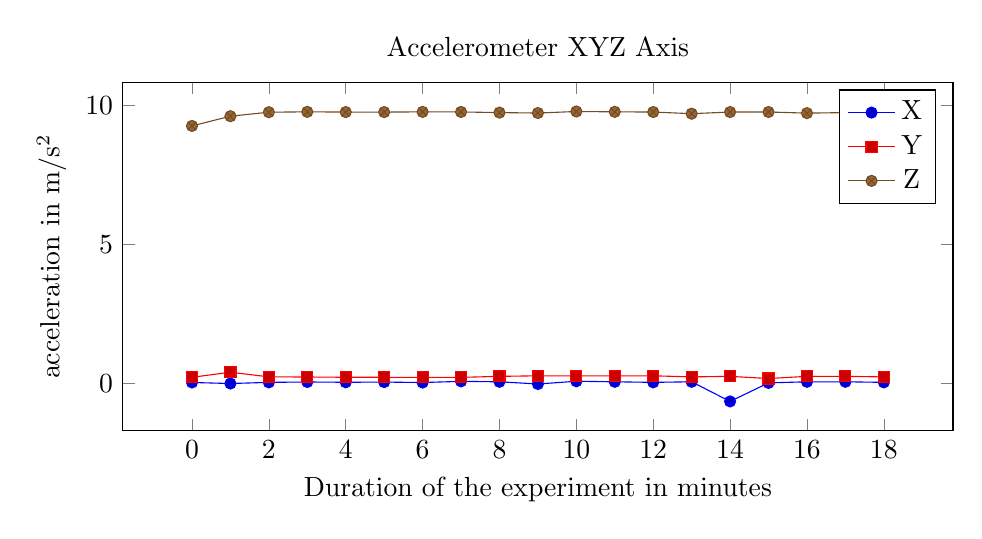
\begin{tikzpicture}
\begin{axis}[
	height=6cm,
	width=\textwidth,
	xlabel=Duration of the experiment in minutes,
	ylabel=acceleration in m/s$^2$,
	title=Accelerometer XYZ Axis,
	unbounded coords=discard],
	
%X
\addplot coordinates {
(0 , 0.0349651822609)
(1 , -0.00309673126316)
(2 , 0.0382930208571)
(3 , 0.0523034957619)
(4 , 0.0420292439048)
(5 , 0.049033425)
(6 , 0.0326879590952)
(7 , 0.0751864109167)
(8 , 0.05883789)
(9 , -0.019607544)
(10 , 0.07846069)
(11 , 0.05883789)
(12 , 0.039230347)
(13 , 0.05883789)
(14 , -0.64723206)
(15 , 0.019607544)
(16 , 0.05883789)
(17 , 0.05883789)
(18 , 0.039230347)
};

%Y
\addplot coordinates {
(0 , 0.220863674783)
(1 , 0.403620667895)
(2 , 0.23722984381)
(3 , 0.231626238095)
(4 , 0.222285678571)
(5 , 0.221095690909)
(6 , 0.217615762857)
(7 , 0.219015755833)
(8 , 0.25497437)
(9 , 0.2745819)
(10 , 0.2745819)
(11 , 0.2745819)
(12 , 0.2745819)
(13 , 0.23536682)
(14 , 0.25497437)
(15 , 0.17651367)
(16 , 0.25497437)
(17 , 0.25497437)
(18 , 0.23536682)
};

%Z
\addplot coordinates {
(0 , 9.26770895652)
(1 , 9.61774347368)
(2 , 9.76181833333)
(3 , 9.77489447619)
(4 , 9.76648904762)
(5 , 9.76563831818)
(6 , 9.77396304762)
(7 , 9.77069233333)
(8 , 9.74780316161)
(9 , 9.73178425312)
(10 , 9.78743477033)
(11 , 9.77489304762)
(12 , 9.76742633556)
(13 , 9.70858834222)
(14 , 9.76742655645)
(15 , 9.76935722354)
(16 , 9.72819595862)
(17 , 9.74780318532)
(18 , 9.70858858813)
};

\addlegendentry{X}
\addlegendentry{Y}
\addlegendentry{Z}
\end{axis}
\end{tikzpicture}
 	\vspace{5 mm}
\end{figure}

\FloatBarrier
\subsection{Light Level}
\begin{figure}[ht]
	\centering
	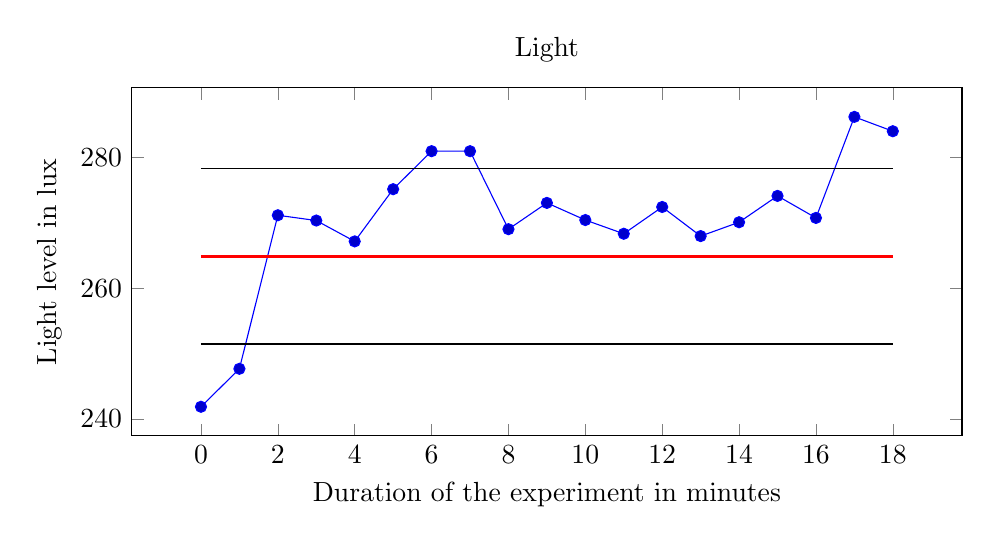
\begin{tikzpicture}
\begin{axis}[
	height=6cm,
	width=\textwidth,
	xlabel=Duration of the experiment in minutes,
	ylabel=Light level in lux,
	title=Light,
	unbounded coords=discard],
	
\addplot coordinates {
(0 , 241.869565217)
(1 , 247.684210526)
(2 , 271.19047619)
(3 , 270.380952381)
(4 , 267.19047619)
(5 , 275.181818182)
(6 , 281.0)
(7 , 281.0)
(8 , 269.056565454)
(9 , 273.082245)
(10 , 270.457685359)
(11 , 268.358045125)
(12 , 272.456782138)
(13 , 268.0)
(14 , 270.121246868)
(15 , 274.154865478)
(16 , 270.782398425)
(17 , 286.252546845)
(18 , 284.054086785)
};

\addplot[mark=none, red, very thick] coordinates {(0, 264.928214098) (18, 264.928214098)};

\addplot[mark=none, black] coordinates {(0, 251.47691699) (18, 251.47691699)};
\addplot[mark=none, black] coordinates {(0, 278.379511206) (18, 278.379511206)};

\end{axis}
\end{tikzpicture}
 	\vspace{5 mm}
\end{figure}

\newpage
\FloatBarrier
\newpage
\subsection{Noise Level}
\begin{figure}[ht]
	\centering
	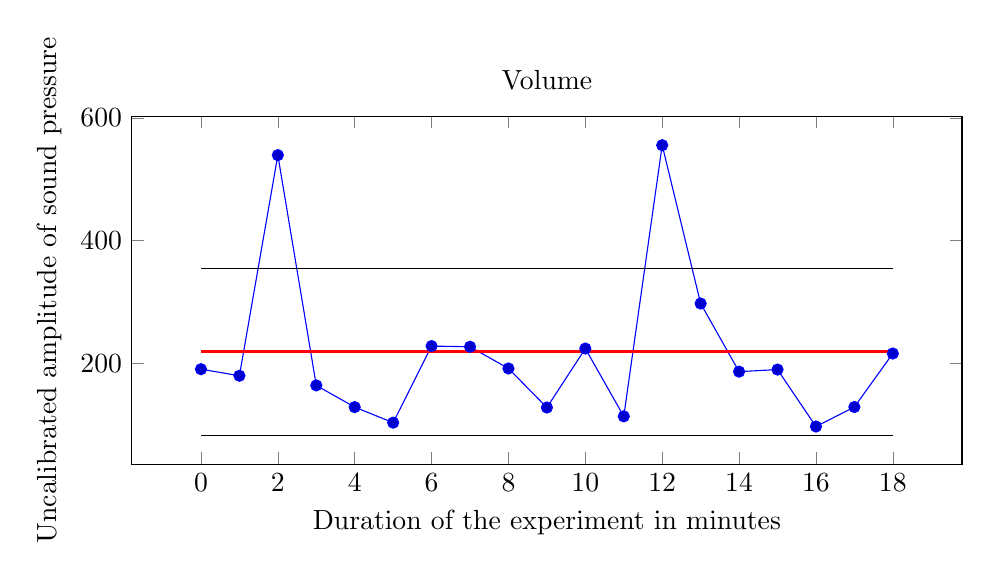
\begin{tikzpicture}
\begin{axis}[
	height=6cm,
	width=\textwidth,
	ylabel=Uncalibrated amplitude of sound pressure,
	xlabel=Duration of the experiment in minutes,
	title=Volume,
	unbounded coords=discard],

\addplot coordinates {
(0 , 190.434782609)
(1 , 179.736842105)
(2 , 539.238095238)
(3 , 164.0)
(4 , 128.619047619)
(5 , 103.318181818)
(6 , 228.095238095)
(7 , 227.0)
(8 , 191.596186522)
(9 , 127.958334583)
(10 , 224.056548712)
(11 , 113.580190875)
(12 , 555.4568753253)
(13 , 297.4565454254)
(14 , 186.4298341674)
(15 , 189.8012096456)
(16 , 97.0)
(17 , 128.8121400108)
(18 , 215.9958225684)
};

\addplot[mark=none, red, very thick] coordinates {(0, 219.063169641) (18, 219.063169641)};

\addplot[mark=none, black] coordinates {(0, 83.0123913636) (18, 83.0123913636)};
\addplot[mark=none, black] coordinates {(0, 355.113947918) (18, 355.113947918)};

\end{axis}
\end{tikzpicture}
 	\vspace{5 mm}
\end{figure}

\FloatBarrier

\subsection{Location}
minute 0 : -3.6881917, 40.4579957
minute 1 : -3.68815341053, 40.4579801474)
from minute 2 : -3.6881432, 40.457976)

Madrid, Spain 

\FloatBarrier
\clearpage
\section{Participant 3}

\subsection{date \& time}
\begin{table}[ht]
  \begin{tabular}{|P{3cm}|P{3cm}|}
	\multicolumn{2}{c}{\textbf{2016-07-28}}    	\\ \hline
    Start Time      			& End Time   					\\ \hline
   \textbf{12:52:44} 	& \textbf{13:04:45}    	\\ \hline
   \multicolumn{2}{c}{Duration}    						\\ \hline
   \multicolumn{2}{c}{\textbf{00:12:01}} 			\\ \hline
  \end{tabular}
  \newline\newline
 \caption{p3: date and time}\label{dandt1}
\end{table}

\subsection{Questions}
\begin{itemize} 
  \item[\Checkmark] Are you a Student?
  \item[\XSolidBrush] Did you work in a team?
  \item[\Checkmark] Did you listen to music?
  \item[\XSolidBrush] Did you feel tired?
  \item[\Checkmark] Did you enjoy the tasks?
  \item[\Checkmark] Did you give all you attention to the tasks?
  \item[\XSolidBrush] Were you distracted during the tasks?
  \item[\XSolidBrush] Did you feel stressed
  \item[\XSolidBrush] Do you think the tasks were easy?  
\end{itemize}


\FloatBarrier
\newpage
\subsection{Accelerometer}

\begin{figure}[ht]
	\centering
	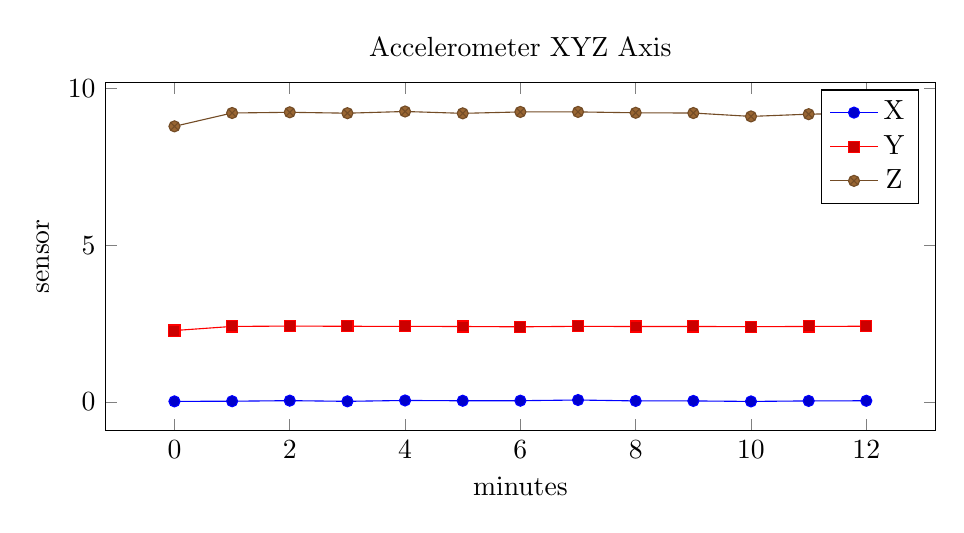
\begin{tikzpicture}
\begin{axis}[
	height=6cm,
	width=\textwidth,
	xlabel=minutes,
	ylabel=sensor,
	title=Accelerometer XYZ Axis,
	unbounded coords=discard],
	
%X
\addplot coordinates {
(0 , 0.019438637881)
(1 , 0.0247400849444)
(2 , 0.0424115735714)
(3 , 0.02101577)
(4 , 0.0486535994286)
(5 , 0.0389057787143)
(6 , 0.041366485)
(7 , 0.0629475533333)
(8 , 0.034117374125)
(9 , 0.033618582)
(10 , 0.0179565136667)
(11 , 0.0341173747143)
(12 , 0.038905777)
};

%Y
\addplot coordinates {
(0 , 2.2777979)
(1 , 2.40836742222)
(2 , 2.42019587143)
(3 , 2.41288974444)
(4 , 2.41164518571)
(5 , 2.40600168571)
(6 , 2.39666241111)
(7 , 2.4114599)
(8 , 2.4058734375)
(9 , 2.40826766667)
(10 , 2.3990899)
(11 , 2.40848141429)
(12 , 2.4145525)
};

%Z
\addplot coordinates {
(0 , 8.7865777619)
(1 , 9.21202333333)
(2 , 9.234265)
(3 , 9.20590511111)
(4 , 9.26008828571)
(5 , 9.20108792857)
(6 , 9.24580855556)
(7 , 9.24680616667)
(8 , 9.2185745)
(9 , 9.21099291667)
(10 , 9.1032535)
(11 , 9.17449528571)
(12 , 9.20391)
};

\addlegendentry{X}
\addlegendentry{Y}
\addlegendentry{Z}
\end{axis}
\end{tikzpicture}
 	\vspace{5 mm}
\end{figure}

\FloatBarrier
\subsection{Light}
\begin{figure}[ht]
	\centering
	\begin{tikzpicture}
\begin{axis}[
	height=6cm,
	width=\textwidth,
	xlabel=minutes,
	ylabel=sensor,
	title=Light,
	unbounded coords=discard],
	
\addplot coordinates {
(0 , 330.986057143)
(1 , 327.141866667)
(2 , 324.539771429)
(3 , 322.701066667)
(4 , 329.208342857)
(5 , 335.669942857)
(6 , 346.047466667)
(7 , 352.541066667)
(8 , 368.9453)
(9 , 374.263066667)
(10 , 355.196133333)
(11 , 340.515885714)
(12 , 332.4064)
};

\end{axis}
\end{tikzpicture}
 	\vspace{5 mm}
\end{figure}

\newpage
\FloatBarrier
\newpage
\subsection{Volume}
\begin{figure}[ht]
	\centering
	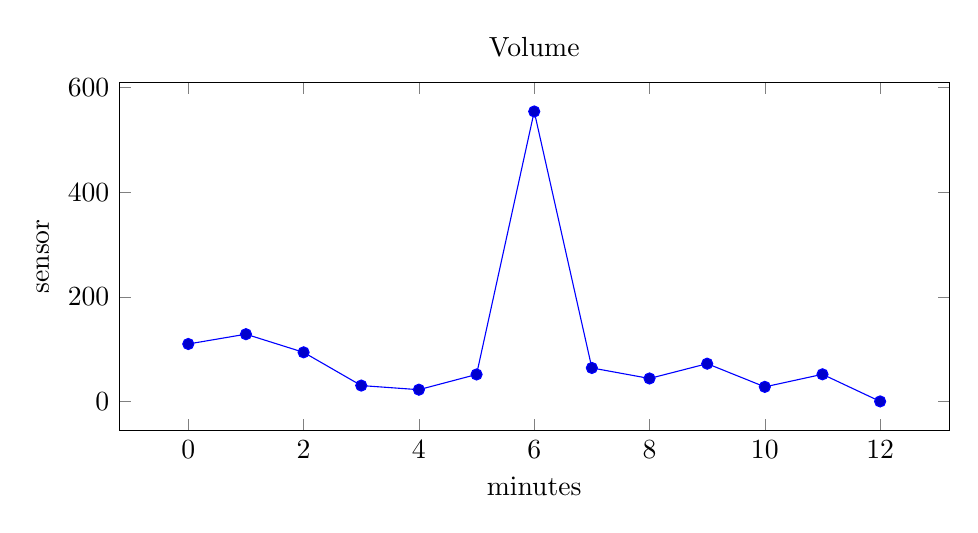
\begin{tikzpicture}
\begin{axis}[
	height=6cm,
	width=\textwidth,
	xlabel=minutes,
	ylabel=sensor,
	title=Volume,
	unbounded coords=discard],

\addplot coordinates {
(0 , 109.80952381)
(1 , 128.555555556)
(2 , 93.8571428571)
(3 , 30.3333333333)
(4 , 22.4285714286)
(5 , 51.5714285714)
(6 , 554.333333333)
(7 , 64.0)
(8 , 43.875)
(9 , 72.1666666667)
(10 , 27.8333333333)
(11 , 51.8571428571)
(12 , 0.0)
};

\end{axis}
\end{tikzpicture}
 	\vspace{5 mm}
\end{figure}

\FloatBarrier
\subsection{Steps}
\begin{figure}[ht]
	\centering
	\begin{tikzpicture}
\begin{axis}[
	height=6cm,
	width=\textwidth,
	xlabel=minutes,
	ylabel=sensor,
	title=Steps,
	unbounded coords=discard],

\addplot coordinates {
(0 , 0.0)
(1 , 0.0)
(2 , 0.0)
(3 , 0.0)
(4 , 0.0)
(5 , 0.0)
(6 , 0.0)
(7 , 0.0)
(8 , 0.0)
(9 , 0.0)
(10 , 0.0)
(11 , 0.0)
(12 , 0.0)
};

\end{axis}
\end{tikzpicture}
 	\vspace{5 mm}
\end{figure}

\newpage
\FloatBarrier

\subsection{Location}
No data gathered

\FloatBarrier
\subsection{Weather}
No data gathered

\FloatBarrier
\clearpage
\section{Participant 4}

%% MK

\subsection{Date \& Time}
\begin{table}[ht]
  \begin{tabular}{|P{3cm}|P{3cm}|}
	\multicolumn{2}{c}{\textbf{2016-08-04}}    	\\ \hline
    Start Time      			& End Time   					\\ \hline
   \textbf{10:20:13} 	& \textbf{11:20:41}    	\\ \hline
   \multicolumn{2}{c}{Duration}    						\\ \hline
   \multicolumn{2}{c}{\textbf{01:00:28}} 			\\ \hline
  \end{tabular}
  \newline\newline
  \caption{P4: Date and Time}\label{dandt4}
\end{table}

\subsection{Questions}
\begin{itemize} 
  \item[\Checkmark] Are you a Student?
  \item[\XSolidBrush] Did you work in a team?
  \item[\XSolidBrush] Did you listen to music?
  \item[\Checkmark] Did you feel tired?
  \item[\Checkmark] Did you enjoy the tasks?
  \item[\XSolidBrush] Did you give all you attention to the tasks?
  \item[\Checkmark] Were you distracted during the tasks?
  \item[\Checkmark] Did you feel stressed
  \item[\XSolidBrush] Do you think the tasks were easy?  
\end{itemize}


\FloatBarrier
\newpage

\subsection{Accelerometer}

\begin{figure}[ht]
	\centering
	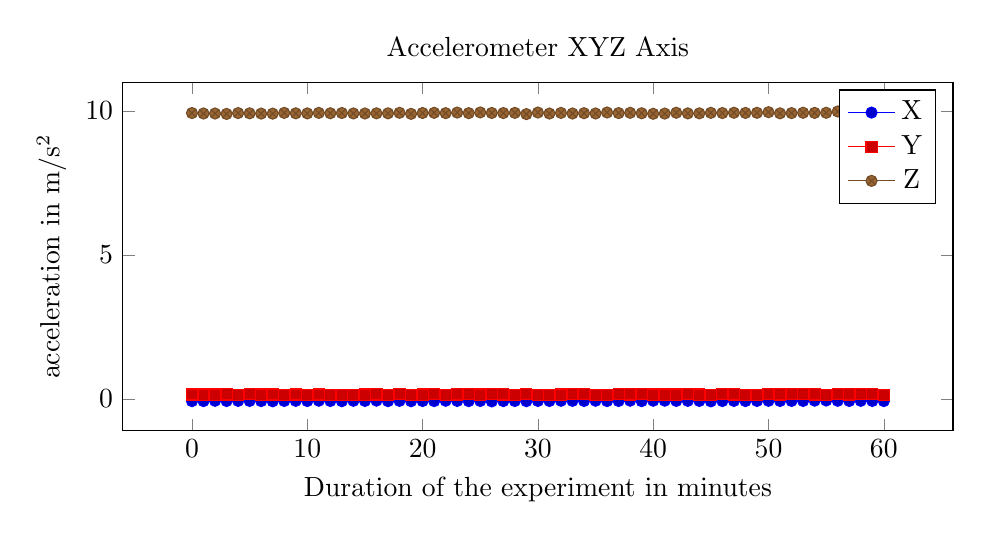
\begin{tikzpicture}
\begin{axis}[
	height=6cm,
	width=\textwidth,
	xlabel=Duration of the experiment in minutes,
	ylabel=acceleration in m/s$^2$,
	title=Accelerometer XYZ Axis,
	unbounded coords=discard],
	
%X
\addplot coordinates {
(0 , -0.0747131762353)
(1 , -0.073247608625)
(2 , -0.063521163625)
(3 , -0.070778586)
(4 , -0.06584054825)
(5 , -0.0672371646667)
(6 , -0.0736217)
(7 , -0.0798067233333)
(8 , -0.0686337833333)
(9 , -0.06434417)
(10 , -0.07122749975)
(11 , -0.0600545593333)
(12 , -0.069282211)
(13 , -0.07631518)
(14 , -0.06299743325)
(15 , -0.0679354745)
(16 , -0.0568622886667)
(17 , -0.07481880275)
(18 , -0.064643445)
(19 , -0.0770134866667)
(20 , -0.0708284676667)
(21 , -0.0723048914)
(22 , -0.061451177)
(23 , -0.0666386146667)
(24 , -0.0737214611667)
(25 , -0.06823475)
(26 , -0.0831985105)
(27 , -0.073621705)
(28 , -0.0700303985)
(29 , -0.07571663)
(30 , -0.06808510825)
(31 , -0.0690328133333)
(32 , -0.06269815775)
(33 , -0.064942722)
(34 , -0.06853402325)
(35 , -0.061052144)
(36 , -0.0724246025)
(37 , -0.0694318475)
(38 , -0.05865794)
(39 , -0.074699092)
(40 , -0.060752869)
(41 , -0.0587576993333)
(42 , -0.066638614)
(43 , -0.065241995)
(44 , -0.0673369215)
(45 , -0.082001406)
(46 , -0.071526772)
(47 , -0.06688800775)
(48 , -0.072723875)
(49 , -0.067636197)
(50 , -0.06314707)
(51 , -0.06958148675)
(52 , -0.0672371633333)
(53 , -0.068035233)
(54 , -0.0580593925)
(55 , -0.0528434535714)
(56 , -0.06254852)
(57 , -0.0688017963684)
(58 , -0.06464344625)
(59 , -0.068234749)
(60 , -0.0725243588333)
};

%Y
\addplot coordinates {
(0 , 0.156256870588)
(1 , 0.15315409)
(2 , 0.15367782375)
(3 , 0.15786767)
(4 , 0.14454993)
(5 , 0.16360378)
(6 , 0.15382746)
(7 , 0.155822623333)
(8 , 0.145846786667)
(9 , 0.155323835)
(10 , 0.15083471)
(11 , 0.155822626667)
(12 , 0.1484405075)
(13 , 0.142455)
(14 , 0.144250655)
(15 , 0.15412673)
(16 , 0.157219246667)
(17 , 0.1415571775)
(18 , 0.160411515)
(19 , 0.147442923333)
(20 , 0.154226496667)
(21 , 0.159214414)
(22 , 0.148240986667)
(23 , 0.157219246667)
(24 , 0.161508855)
(25 , 0.154126735)
(26 , 0.165499195)
(27 , 0.15682021)
(28 , 0.15203181)
(29 , 0.187047005)
(30 , 0.143352825)
(31 , 0.15003664)
(32 , 0.1550245625)
(33 , 0.16011224)
(34 , 0.1593640525)
(35 , 0.15023616)
(36 , 0.14514848)
(37 , 0.16071079)
(38 , 0.15741876)
(39 , 0.162207164)
(40 , 0.15502456)
(41 , 0.15522408)
(42 , 0.153627943333)
(43 , 0.17238252)
(44 , 0.153528185)
(45 , 0.14584679)
(46 , 0.16190789)
(47 , 0.15816695)
(48 , 0.15263036)
(49 , 0.14754268)
(50 , 0.16011224)
(51 , 0.157269125)
(52 , 0.159812963333)
(53 , 0.165997983333)
(54 , 0.15831659)
(55 , 0.147499927143)
(56 , 0.172981075)
(57 , 0.157733788421)
(58 , 0.1634042675)
(59 , 0.1726818)
(60 , 0.140360076667)
};

%Z
\addplot coordinates {
(0 , 9.92474058824)
(1 , 9.9079546875)
(2 , 9.9084784375)
(3 , 9.89433775)
(4 , 9.923517)
(5 , 9.914589)
(6 , 9.905411)
(7 , 9.90421416667)
(8 , 9.93035066667)
(9 , 9.914988)
(10 , 9.91244375)
(11 , 9.930351)
(12 , 9.9172325)
(13 , 9.925762)
(14 , 9.9112465)
(15 , 9.9093015)
(16 , 9.914589)
(17 , 9.91423975)
(18 , 9.9332435)
(19 , 9.89643233333)
(20 , 9.92596133333)
(21 , 9.9329444)
(22 , 9.92097333333)
(23 , 9.940925)
(24 , 9.92167158333)
(25 , 9.9455135)
(26 , 9.9275575)
(27 , 9.92396633333)
(28 , 9.93055)
(29 , 9.8877535)
(30 , 9.94282025)
(31 , 9.907406)
(32 , 9.92965225)
(33 , 9.908703)
(34 , 9.919028)
(35 , 9.90940133333)
(36 , 9.9437185)
(37 , 9.923218)
(38 , 9.932944)
(39 , 9.9166634)
(40 , 9.8985275)
(41 , 9.90640833333)
(42 , 9.935538)
(43 , 9.9128925)
(44 , 9.91379075)
(45 , 9.931947)
(46 , 9.9242655)
(47 , 9.9341415)
(48 , 9.9284555)
(49 , 9.932645)
(50 , 9.954492)
(51 , 9.91409)
(52 , 9.92296833333)
(53 , 9.93414133333)
(54 , 9.930101)
(55 , 9.93345728571)
(56 , 9.9787335)
(57 , 9.92550976316)
(58 , 9.91049875)
(59 , 9.9203745)
(60 , 9.92167166667)
};

\addlegendentry{X}
\addlegendentry{Y}
\addlegendentry{Z}
\end{axis}
\end{tikzpicture}
 	\vspace{5 mm}
\end{figure}

\FloatBarrier
\subsection{Light Level}
\begin{figure}[ht]
	\centering
	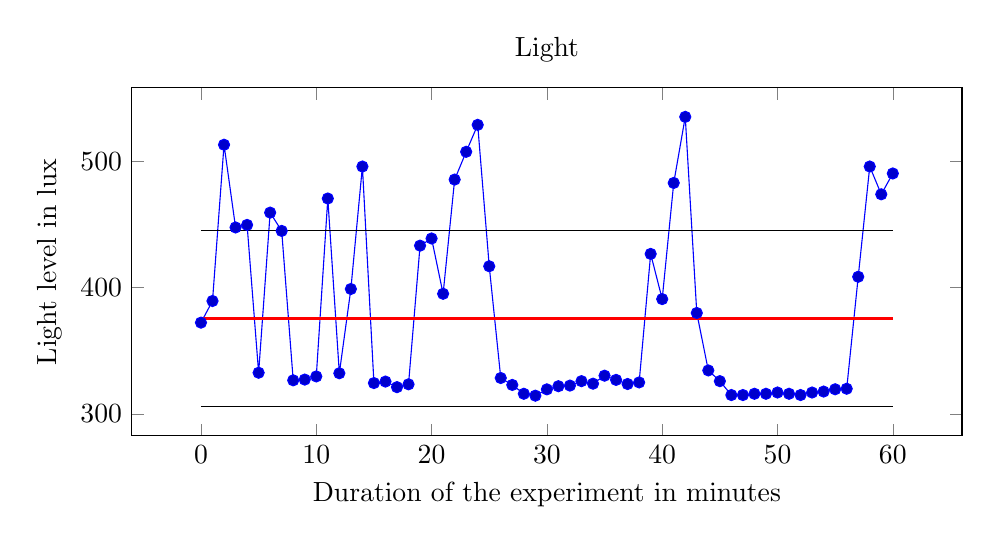
\begin{tikzpicture}
\begin{axis}[
	height=6cm,
	width=\textwidth,
	xlabel=Duration of the experiment in minutes,
	ylabel=Light level in lux,
	title=Light,
	unbounded coords=discard],
	
\addplot coordinates {
(0 , 372.352941176)
(1 , 389.5)
(2 , 513.25)
(3 , 447.75)
(4 , 449.75)
(5 , 332.666666667)
(6 , 459.5)
(7 , 445.0)
(8 , 326.666666667)
(9 , 327.25)
(10 , 329.75)
(11 , 470.666666667)
(12 , 332.25)
(13 , 399.0)
(14 , 496.0)
(15 , 324.5)
(16 , 325.666666667)
(17 , 321.25)
(18 , 323.5)
(19 , 433.333333333)
(20 , 439.0)
(21 , 395.2)
(22 , 485.666666667)
(23 , 507.666666667)
(24 , 529.0)
(25 , 417.0)
(26 , 328.5)
(27 , 323.0)
(28 , 316.0)
(29 , 314.5)
(30 , 319.5)
(31 , 322.0)
(32 , 322.5)
(33 , 326.0)
(34 , 324.0)
(35 , 330.333333333)
(36 , 327.0)
(37 , 323.75)
(38 , 325.0)
(39 , 426.8)
(40 , 391.0)
(41 , 483.0)
(42 , 535.333333333)
(43 , 380.0)
(44 , 334.5)
(45 , 326.0)
(46 , 315.0)
(47 , 315.0)
(48 , 316.0)
(49 , 316.0)
(50 , 317.0)
(51 , 316.0)
(52 , 315.0)
(53 , 317.0)
(54 , 317.75)
(55 , 319.571428571)
(56 , 320.0)
(57 , 408.684210526)
(58 , 496.0)
(59 , 474.0)
(60 , 490.5)
};

\addplot[mark=none, red, very thick] coordinates {(0, 375.580976338) (60, 375.580976338)};

\addplot[mark=none, black] coordinates {(0, 305.697485999) (60, 305.697485999)};
\addplot[mark=none, black] coordinates {(0, 445.464466676) (60, 445.464466676)};


\end{axis}
\end{tikzpicture}
 	\vspace{5 mm}
\end{figure}

\newpage
\FloatBarrier
\newpage
\subsection{Noise Level}
\begin{figure}[ht]
	\centering
	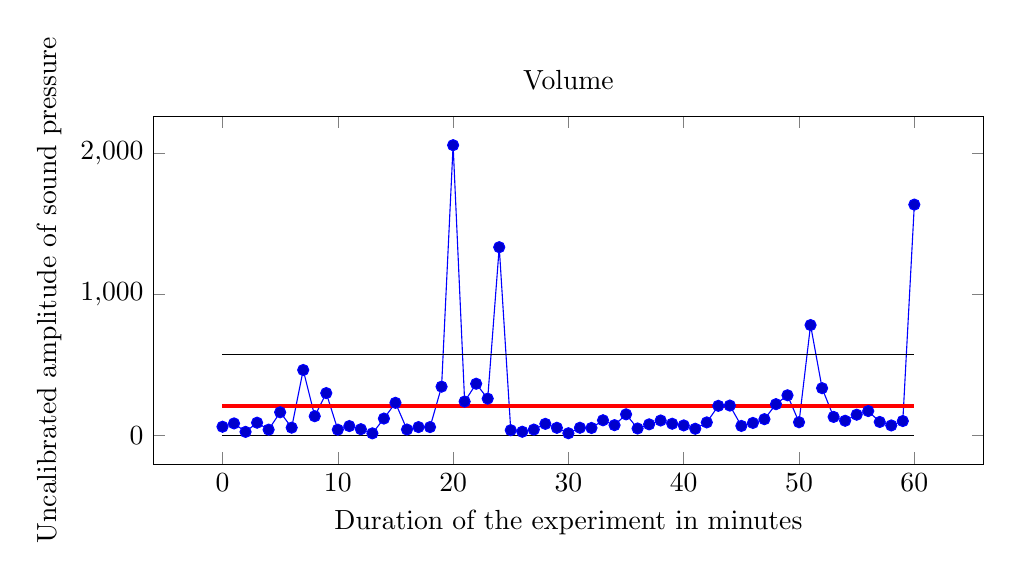
\begin{tikzpicture}
\begin{axis}[
	height=6cm,
	width=\textwidth,
	ylabel=Uncalibrated amplitude of sound pressure,
	xlabel=Duration of the experiment in minutes,
	title=Volume,
	unbounded coords=discard],

\addplot coordinates {
(0 , 59.5882352941)
(1 , 83.125)
(2 , 23.0)
(3 , 88.25)
(4 , 38.75)
(5 , 162.333333333)
(6 , 53.0)
(7 , 462.666666667)
(8 , 134.333333333)
(9 , 298.5)
(10 , 38.5)
(11 , 64.3333333333)
(12 , 42.0)
(13 , 12.5)
(14 , 117.75)
(15 , 229.5)
(16 , 39.6666666667)
(17 , 57.0)
(18 , 57.0)
(19 , 344.333333333)
(20 , 2060.0)
(21 , 238.6)
(22 , 365.0)
(23 , 259.0)
(24 , 1335.16666667)
(25 , 35.0)
(26 , 24.0)
(27 , 39.3333333333)
(28 , 80.0)
(29 , 52.0)
(30 , 13.25)
(31 , 52.3333333333)
(32 , 50.75)
(33 , 105.5)
(34 , 70.75)
(35 , 147.666666667)
(36 , 47.0)
(37 , 76.5)
(38 , 104.0)
(39 , 80.8)
(40 , 69.0)
(41 , 45.1666666667)
(42 , 90.3333333333)
(43 , 208.0)
(44 , 210.0)
(45 , 65.3333333333)
(46 , 86.5)
(47 , 113.25)
(48 , 220.0)
(49 , 283.0)
(50 , 91.5)
(51 , 782.0)
(52 , 333.666666667)
(53 , 129.333333333)
(54 , 102.0)
(55 , 145.0)
(56 , 171.0)
(57 , 93.5789473684)
(58 , 68.75)
(59 , 100.0)
(60 , 1637.83333333)
};

\addplot[mark=none, red, very thick] coordinates {(0, 208.000418295) (60, 208.000418295)};

\addplot[mark=none, black] coordinates {(0, 0) (60, 0)};
\addplot[mark=none, black] coordinates {(0, 571.657643466) (60, 571.657643466)};

\end{axis}
\end{tikzpicture}
 	\vspace{5 mm}
\end{figure}

\FloatBarrier

\subsection{Location}
53.3437734, -6.2510318

Dublin, Ireland 

\FloatBarrier
\clearpage
\section{Participant 5}

%HS

\subsection{Date \& Time}
\begin{table}[ht]
  \begin{tabular}{|P{3cm}|P{3cm}|}
	\multicolumn{2}{c}{\textbf{2016-08-09}}    	\\ \hline
    Start Time      			& End Time   					\\ \hline
   \textbf{15:49:28} 	& \textbf{17:20:58}    	\\ \hline
   \multicolumn{2}{c}{Duration}    						\\ \hline
   \multicolumn{2}{c}{\textbf{01:31:30}} 			\\ \hline
  \end{tabular}
  \newline\newline
  \caption{P5: Date and Time}\label{dandt5}
\end{table}

\FloatBarrier

\subsection{Questions}
\begin{itemize} 
  \item[\Checkmark] Are you a Student?
  \item[\XSolidBrush] Did you work in a team?
  \item[\XSolidBrush] Did you listen to music?
  \item[\XSolidBrush] Did you feel tired?
  \item[\Checkmark] Did you enjoy the tasks?
  \item[\Checkmark] Did you give all you attention to the tasks?
  \item[\XSolidBrush] Were you distracted during the tasks?
  \item[\XSolidBrush] Did you feel stressed
  \item[\XSolidBrush] Do you think the tasks were easy?  
\end{itemize}


\FloatBarrier
\newpage
\subsection{Accelerometer}

\begin{figure}[ht]
	\centering
	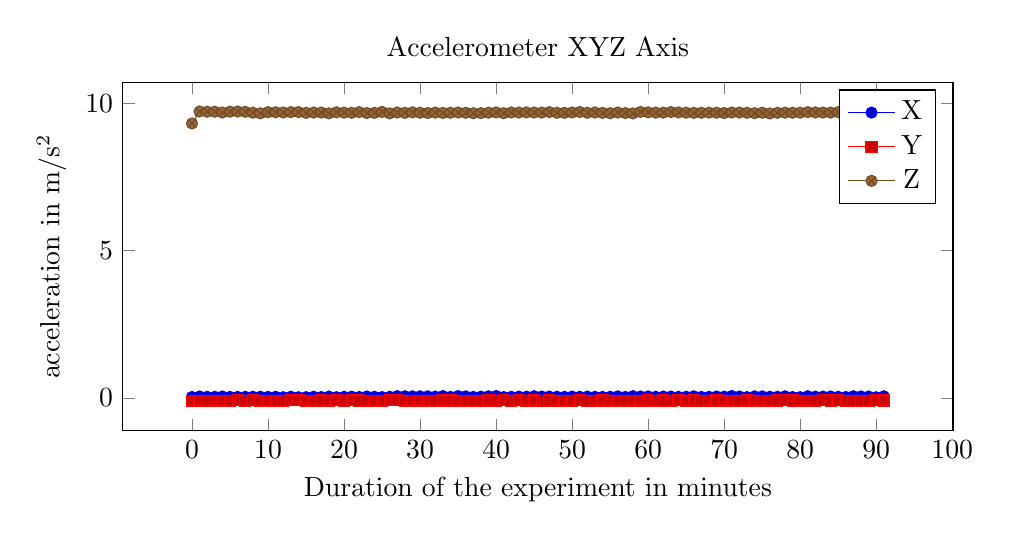
\begin{tikzpicture}
\begin{axis}[
	height=6cm,
	width=\textwidth,
	xlabel=Duration of the experiment in minutes,
	ylabel=acceleration in m/s$^2$,
	title=Accelerometer XYZ Axis,
	unbounded coords=discard],
	
%X
\addplot coordinates {
(0 , 0.028624852325)
(1 , 0.0456503159435)
(2 , 0.0345175602857)
(3 , 0.0348083495)
(4 , 0.04493713425)
(5 , 0.03185272225)
(6 , 0.032054901)
(7 , 0.0333658853333)
(8 , 0.03527832025)
(9 , 0.037109375)
(10 , 0.0322875975)
(11 , 0.036422729)
(12 , 0.02068481454)
(13 , 0.0372229681111)
(14 , 0.0187072753833)
(15 , 0.02278137175)
(16 , 0.0373102818333)
(17 , 0.0263108474615)
(18 , 0.0425605775)
(19 , 0.021026611)
(20 , 0.0350392652833)
(21 , 0.0383300785)
(22 , 0.0275421141)
(23 , 0.0451100666667)
(24 , 0.035198212)
(25 , 0.023899078475)
(26 , 0.035690308)
(27 , 0.05596923825)
(28 , 0.05286331185)
(29 , 0.0494931539167)
(30 , 0.0507286924444)
(31 , 0.0508575438)
(32 , 0.0422706605)
(33 , 0.0589447026667)
(34 , 0.03134918226)
(35 , 0.0602783198)
(36 , 0.0494422905)
(37 , 0.031689962)
(38 , 0.039909362)
(39 , 0.050775147)
(40 , 0.0615295414)
(41 , 0.0245971678667)
(42 , 0.0336181642)
(43 , 0.04070663425)
(44 , 0.038182577)
(45 , 0.05458831725)
(46 , 0.043797811)
(47 , 0.0426910398)
(48 , 0.0372436522)
(49 , 0.0326446532)
(50 , 0.0426849356)
(51 , 0.0350494386667)
(52 , 0.04183197075)
(53 , 0.03400802625)
(54 , 0.030904134)
(55 , 0.034921264)
(56 , 0.049016317)
(57 , 0.0298919676667)
(58 , 0.055935669)
(59 , 0.045284271)
(60 , 0.0474853525)
(61 , 0.0355326333333)
(62 , 0.04415130625)
(63 , 0.04241180425)
(64 , 0.0335184733333)
(65 , 0.0360717774)
(66 , 0.05042648375)
(67 , 0.03061294525)
(68 , 0.0333030008182)
(69 , 0.0442055152105)
(70 , 0.040286255)
(71 , 0.0616607675)
(72 , 0.0454444895)
(73 , 0.024180095)
(74 , 0.049064636)
(75 , 0.0488922114)
(76 , 0.03613281275)
(77 , 0.03391647325)
(78 , 0.0513407386667)
(79 , 0.0258255005)
(80 , 0.023609161425)
(81 , 0.054763794)
(82 , 0.0396626796667)
(83 , 0.04229354875)
(84 , 0.0447021485)
(85 , 0.0336486822)
(86 , 0.0279922485)
(87 , 0.0545578005)
(88 , 0.0470581055)
(89 , 0.0445327755)
(90 , 0.019207001)
(91 , 0.05170059225)
};

%Y
\addplot coordinates {
(0 , -0.09772237125)
(1 , -0.108810424783)
(2 , -0.103489468571)
(3 , -0.105393982)
(4 , -0.1029891965)
(5 , -0.09886169375)
(6 , -0.087383271)
(7 , -0.0943857833333)
(8 , -0.08496475)
(9 , -0.0982716866667)
(10 , -0.09655761625)
(11 , -0.0961120602)
(12 , -0.107305908)
(13 , -0.081837973)
(14 , -0.0802561431667)
(15 , -0.095504761)
(16 , -0.0975189198333)
(17 , -0.0929166354615)
(18 , -0.097572326)
(19 , -0.0717506415)
(20 , -0.0957183841667)
(21 , -0.08687210025)
(22 , -0.09144973825)
(23 , -0.09747823)
(24 , -0.101642611)
(25 , -0.1035652175)
(26 , -0.066518148)
(27 , -0.08568573)
(28 , -0.10135345475)
(29 , -0.102905273208)
(30 , -0.10242886)
(31 , -0.1043487568)
(32 , -0.102169036)
(33 , -0.091405232)
(34 , -0.09143066375)
(35 , -0.1044128416)
(36 , -0.10267639)
(37 , -0.1101964315)
(38 , -0.1020584125)
(39 , -0.0895660396)
(40 , -0.1017395028)
(41 , -0.0832926433333)
(42 , -0.102542115)
(43 , -0.087623596)
(44 , -0.0957692433333)
(45 , -0.09049987875)
(46 , -0.0987981168333)
(47 , -0.090505982)
(48 , -0.0970825196)
(49 , -0.095925903)
(50 , -0.103506469)
(51 , -0.087066651)
(52 , -0.10188675)
(53 , -0.10551452675)
(54 , -0.0904235846667)
(55 , -0.0952545168)
(56 , -0.100504556667)
(57 , -0.105763753333)
(58 , -0.098510743)
(59 , -0.104553225)
(60 , -0.089305879)
(61 , -0.120956418667)
(62 , -0.0916442855)
(63 , -0.105182646)
(64 , -0.082397462)
(65 , -0.101950074)
(66 , -0.09177398725)
(67 , -0.0966796875)
(68 , -0.0961914064545)
(69 , -0.0925381308421)
(70 , -0.1081848152)
(71 , -0.0940208435)
(72 , -0.09459114075)
(73 , -0.0914408366667)
(74 , -0.095474245)
(75 , -0.101541138)
(76 , -0.110935209)
(77 , -0.087963105)
(78 , -0.086324055)
(79 , -0.090545655)
(80 , -0.11132431)
(81 , -0.09964752125)
(82 , -0.12154134)
(83 , -0.07924652)
(84 , -0.0934127799)
(85 , -0.0864471432)
(86 , -0.09584426875)
(87 , -0.099739075)
(88 , -0.1060752875)
(89 , -0.09546661375)
(90 , -0.0802040115)
(91 , -0.0905571)
};

%Z
\addplot coordinates {
(0 , 9.3104775)
(1 , 9.71597156522)
(2 , 9.70799707143)
(3 , 9.7079117)
(4 , 9.68053425)
(5 , 9.71026225)
(6 , 9.715645)
(7 , 9.70654266667)
(8 , 9.675411)
(9 , 9.65371166667)
(10 , 9.693695)
(11 , 9.6893708)
(12 , 9.6818605)
(13 , 9.69282183333)
(14 , 9.69518283333)
(15 , 9.669311625)
(16 , 9.68030308333)
(17 , 9.67978007692)
(18 , 9.65250425)
(19 , 9.68883525)
(20 , 9.67687475)
(21 , 9.6719855)
(22 , 9.695724375)
(23 , 9.66287733333)
(24 , 9.66836925)
(25 , 9.70105)
(26 , 9.651494)
(27 , 9.681896)
(28 , 9.66984335)
(29 , 9.68622652083)
(30 , 9.67309044444)
(31 , 9.6627592)
(32 , 9.6778755)
(33 , 9.66750083333)
(34 , 9.673275)
(35 , 9.6826139)
(36 , 9.671501)
(37 , 9.65692133333)
(38 , 9.661518)
(39 , 9.6754394)
(40 , 9.6855011)
(41 , 9.657328)
(42 , 9.6824404)
(43 , 9.68023675)
(44 , 9.684133)
(45 , 9.68102275)
(46 , 9.67905545833)
(47 , 9.6964352)
(48 , 9.6722078)
(49 , 9.6715148)
(50 , 9.6816741)
(51 , 9.698008)
(52 , 9.6722985)
(53 , 9.682353875)
(54 , 9.669093)
(55 , 9.6570252)
(56 , 9.68032066667)
(57 , 9.66158566667)
(58 , 9.6507874)
(59 , 9.69986325)
(60 , 9.68689325)
(61 , 9.67655433333)
(62 , 9.67766575)
(63 , 9.698765)
(64 , 9.68428016667)
(65 , 9.6757873)
(66 , 9.670021125)
(67 , 9.67202375)
(68 , 9.67732095455)
(69 , 9.67484878947)
(70 , 9.6626556)
(71 , 9.68144225)
(72 , 9.68019875)
(73 , 9.67266333333)
(74 , 9.65867975)
(75 , 9.6737824)
(76 , 9.648448875)
(77 , 9.671032)
(78 , 9.67692066667)
(79 , 9.674061)
(80 , 9.675293)
(81 , 9.6954535)
(82 , 9.68317666667)
(83 , 9.679886)
(84 , 9.677974)
(85 , 9.6936248)
(86 , 9.65489175)
(87 , 9.67543025)
(88 , 9.66282675)
(89 , 9.66626375)
(90 , 9.68290325)
(91 , 9.6799165)
};

\addlegendentry{X}
\addlegendentry{Y}
\addlegendentry{Z}
\end{axis}
\end{tikzpicture}
 	\vspace{5 mm}
\end{figure}

\FloatBarrier
\subsection{Light Level}
\begin{figure}[ht]
	\centering
	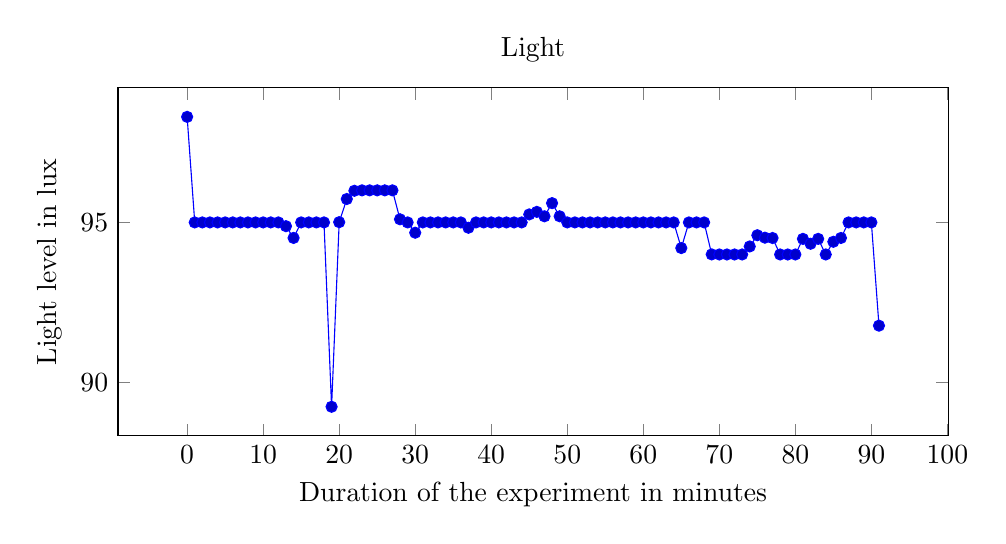
\begin{tikzpicture}
\begin{axis}[
	height=6cm,
	width=\textwidth,
	xlabel=Duration of the experiment in minutes,
	ylabel=Light level in lux,
	title=Light,
	unbounded coords=discard],
	
\addplot coordinates {
(0 , 98.2916666667)
(1 , 95.0)
(2 , 95.0)
(3 , 95.0)
(4 , 95.0)
(5 , 95.0)
(6 , 95.0)
(7 , 95.0)
(8 , 95.0)
(9 , 95.0)
(10 , 95.0)
(11 , 95.0)
(12 , 95.0)
(13 , 94.8825577778)
(14 , 94.5164273333)
(15 , 95.0)
(16 , 95.0)
(17 , 95.0)
(18 , 95.0)
(19 , 89.25)
(20 , 95.0078283333)
(21 , 95.7297625)
(22 , 95.986889)
(23 , 96.0)
(24 , 96.0)
(25 , 96.0)
(26 , 96.0)
(27 , 96.0)
(28 , 95.0976655)
(29 , 95.0)
(30 , 94.678594)
(31 , 95.0)
(32 , 95.0)
(33 , 95.0)
(34 , 95.0)
(35 , 95.0)
(36 , 95.0)
(37 , 94.8333333333)
(38 , 95.0)
(39 , 95.0)
(40 , 95.0)
(41 , 95.0)
(42 , 95.0)
(43 , 95.0)
(44 , 95.0)
(45 , 95.25)
(46 , 95.3285295)
(47 , 95.190542)
(48 , 95.601148)
(49 , 95.190604)
(50 , 95.0)
(51 , 95.0)
(52 , 95.0)
(53 , 95.0)
(54 , 95.0)
(55 , 95.0)
(56 , 95.0)
(57 , 95.0)
(58 , 95.0)
(59 , 95.0)
(60 , 95.0)
(61 , 95.0)
(62 , 95.0)
(63 , 95.0)
(64 , 95.0)
(65 , 94.2)
(66 , 95.0)
(67 , 95.0)
(68 , 95.0)
(69 , 94.0025184211)
(70 , 94.0)
(71 , 94.0)
(72 , 94.0)
(73 , 94.0)
(74 , 94.25)
(75 , 94.6)
(76 , 94.524485)
(77 , 94.5133925)
(78 , 94.0)
(79 , 94.0)
(80 , 94.0)
(81 , 94.48627)
(82 , 94.3333333333)
(83 , 94.486889)
(84 , 94.0)
(85 , 94.3959052)
(86 , 94.5150075)
(87 , 95.0)
(88 , 95.0)
(89 , 95.0)
(90 , 95.0)
(91 , 91.78003)
};

\end{axis}
\end{tikzpicture}
 	\vspace{5 mm}
\end{figure}

\newpage
\FloatBarrier
\newpage
\subsection{Noise Level}
\begin{figure}[ht]
	\centering
	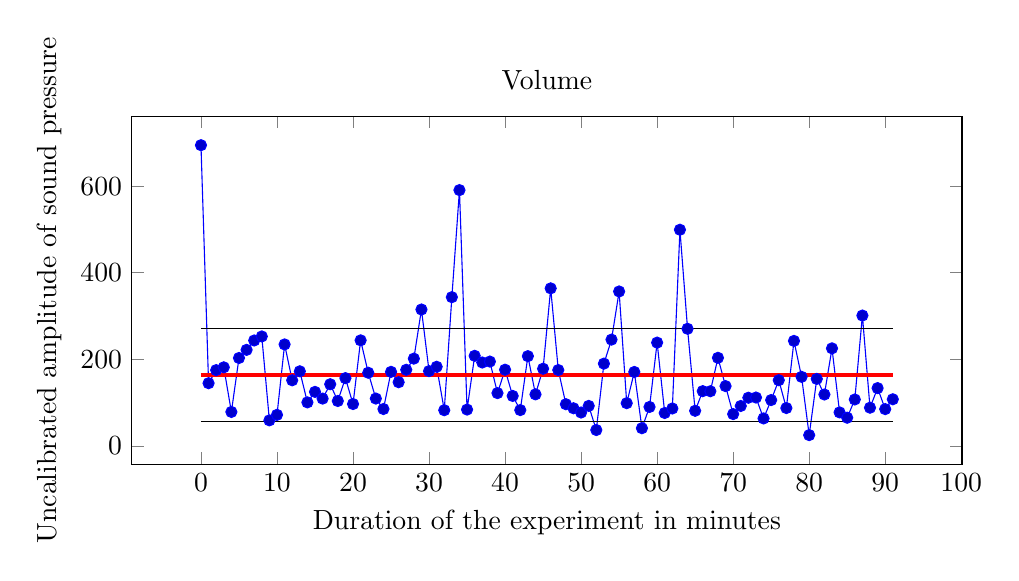
\begin{tikzpicture}
\begin{axis}[
	height=6cm,
	width=\textwidth,
	ylabel=Uncalibrated amplitude of sound pressure,
	xlabel=Duration of the experiment in minutes,
	title=Volume,
	unbounded coords=discard],

\addplot coordinates {
(0 , 694.416666667)
(1 , 145.086956522)
(2 , 175.285714286)
(3 , 181.7)
(4 , 78.75)
(5 , 203.25)
(6 , 222.0)
(7 , 243.666666667)
(8 , 253.0)
(9 , 59.3333333333)
(10 , 72.0)
(11 , 234.6)
(12 , 151.8)
(13 , 172.555555556)
(14 , 100.833333333)
(15 , 125.0)
(16 , 109.5)
(17 , 142.692307692)
(18 , 104.0)
(19 , 156.75)
(20 , 97.0)
(21 , 244.0)
(22 , 169.25)
(23 , 109.666666667)
(24 , 85.5)
(25 , 171.25)
(26 , 147.333333333)
(27 , 176.0)
(28 , 201.8)
(29 , 315.166666667)
(30 , 173.0)
(31 , 183.0)
(32 , 82.75)
(33 , 343.666666667)
(34 , 590.75)
(35 , 84.2)
(36 , 208.25)
(37 , 192.833333333)
(38 , 195.0)
(39 , 122.2)
(40 , 176.2)
(41 , 115.666666667)
(42 , 83.0)
(43 , 207.5)
(44 , 119.333333333)
(45 , 178.5)
(46 , 364.0)
(47 , 175.4)
(48 , 96.6)
(49 , 87.2)
(50 , 77.4)
(51 , 92.6666666667)
(52 , 37.0)
(53 , 190.25)
(54 , 245.666666667)
(55 , 356.8)
(56 , 99.0)
(57 , 171.0)
(58 , 41.2)
(59 , 90.25)
(60 , 238.75)
(61 , 76.3333333333)
(62 , 86.75)
(63 , 499.25)
(64 , 270.666666667)
(65 , 81.4)
(66 , 126.75)
(67 , 126.5)
(68 , 203.636363636)
(69 , 138.368421053)
(70 , 73.8)
(71 , 92.5)
(72 , 111.5)
(73 , 112.0)
(74 , 63.75)
(75 , 106.2)
(76 , 152.0)
(77 , 87.75)
(78 , 242.666666667)
(79 , 159.75)
(80 , 25.25)
(81 , 155.0)
(82 , 119.0)
(83 , 225.5)
(84 , 77.7)
(85 , 65.4)
(86 , 107.5)
(87 , 301.25)
(88 , 88.5)
(89 , 133.75)
(90 , 85.25)
(91 , 108.0)
};

\addplot[mark=none, red, very thick] coordinates {(0, 163.759695494) (91, 163.759695494)};

\addplot[mark=none, black] coordinates {(0, 56.1651969983) (91, 56.1651969983)};
\addplot[mark=none, black] coordinates {(0, 271.354193989) (91, 271.354193989)};

\end{axis}
\end{tikzpicture}
 	\vspace{5 mm}
\end{figure}

\FloatBarrier

\subsection{Location}
-6.250537, 53.3437789

Dublin, Ireland

\FloatBarrier
\end{appendix}

%\addcontentsline {toc}{chapter}{Bibliography}     %% Force Bibliography to appear in contents
%\addcontentsline{toc}{section}{References}

%\begin{thebibliography}{ieeetr} 
\bibliography{references}
\bibliographystyle{plain}
%\end{thebibliography}      

\end{document}